% Important:  
% 1. single spacing before introduction chapter..
% 2. double spacing from intro chapter ..
% 3. modify size of page output ..
% 4. modify documentclass option ..

% Test dataset:
% 1. fuel (small)
% 2. hemoglobin (large)
% 3. ventricle (large)
% 4. MRIHead (very large)
% 5. vh4 (middle)


% TODO: describe the method on construting contour tree

% TODO: include bongbong's paper <time-varying contour topology> 
% as a part of reference

% TODO: improve images

% TODO: create image for performance illustration

% TODO: improve the background section in cell triangulation chapter ...

% TODO: improve cell triangulation section.. which is very important about
% the contribution of this thesis

% TODO: write something about volume rendering .. where a comparison with 
% isosurface extraction method can be made

% TODO: complete the result chapter
% TODO: complete the conclusion chapter

% TODO: test the program on Windows with more processors !!!

% \documentclass[12pt, b5paper]{report}
\documentclass[11pt, b5paper]{report}
\usepackage{pdfpages}
\usepackage{graphicx}
\usepackage{float}
\usepackage{subfig}
\usepackage{multirow}
\usepackage[ruled, linesnumbered]{algorithm2e}
\usepackage{pslatex}
\usepackage{amsmath}
% \usepackage[cm]{fullpage}
\usepackage[margin=2.5cm]{geometry}
\usepackage{lscape}
\usepackage{kotex}
% \pagestyle{plain}
\usepackage{setspace}

\newcommand{\enumeratefix}[1][
\setlength{\parskip}{0pt}
\setlength{\parsep}{0pt}
\setlength{\topsep}{0pt}
\setlength{\itemsep}{0pt}
]{#1}

\singlespacing{}

% \onehalfspacing{}
% \doublespacing{}

% \usepackage{titletoc}
% \titlecontents*{chapter}[0.0em]{\normalsize}{Chapter \thecontentslabel. }{}{\hfill \hspace{5pt} \thecontentspage}[  \\ ]
% \titleformat{\chapter}[display]{hformati}{hlabel i}{hsepi}{hbeforei}[hafter i]

% \parskip 7.2pt

% \pdfpagewidth 8.5in
% \pdfpageheight 11in 
% \pdfpagewidth 18cm
% \pdfpageheight 25.5cm

% ------------------------------
% ------------------------------
% ------------------------------
% ------------------------------
% \documentclass[12pt]{report}
% \usepackage{pdfpages}
% \usepackage{graphicx}
% \usepackage{float}
% \usepackage{subfig}
% \usepackage[ruled, linesnumbered]{algorithm2e}
% \usepackage{pslatex}
% \usepackage{amsmath}
% % \usepackage[cm]{fullpage}
% \usepackage[margin=2.5cm]{geometry}
% % \pagestyle{plain}
% \usepackage{setspace}
% % \singlespacing{}
% % \onehalfspacing{}
% \doublespacing{}

% \parskip 7.2pt

% % \pdfpagewidth 8.5in
% % \pdfpageheight 11in 
% \pdfpagewidth 18cm
% \pdfpageheight 25.5cm
% ------------------------------
% ------------------------------
% ------------------------------
% ------------------------------


% \setlength\topmargin{0in}
% \setlength\headheight{0in}
% \setlength\headsep{0in}
% % \setlength\textheight{9in}
% % \setlength\textwidth{6.5in}
% \setlength\textheight{8in}
% \setlength\textwidth{5in}
% \setlength\oddsidemargin{0in}
% \setlength\evensidemargin{0in}
% \setlength\parindent{0.25in}

% -----------------------------------------------------------------------------

\title{Hybrid Acceleration for Interest-based \\ 
  Contour Component Extraction}
\author{Liangfu Chen}
\date{\today}

\begin{document}

% % \maketitle

% \begin{titlepage}
%     \singlespacing{}
%   \begin{center}
%     \Large{ $116^{\mathrm{th}}$ Master's Thesis } \\[1cm]
%     \Huge{\textbf{Hybrid Acceleration for Interest-based \\ 
%         Contour Component Extraction}}\\[8cm]
%     \Large{\textbf{February 2012}}
%     \vfill
%     % \large{\month \year}\\[5cm]
%     \huge{\textbf{The Graduate School}\\
%     \textbf{Chung-Ang University}}\\
%     \Large{\textbf{School of Computer Science \& Engineering}\\
%     \textbf{Liangfu Chen}}\\[1cm]
%   \end{center}
% \end{titlepage}

% % empty new page
% \newpage{}
% \thispagestyle{empty}
% \mbox{}

\includepdf[pages=1-3]{cau-thesis.pdf}
% \includepdf[page=2]{cau-thesis.pdf}
% \includepdf[page=3]{cau-thesis.pdf}

% \begin{titlepage}
%   \singlespacing{}
%   \begin{center}
%     \Large{ $116^{\mathrm{th}}$ Master's Thesis } \\[1cm]
%     \Huge{{Hybrid Acceleration for Interest-based \\ 
%         Contour Component Extraction}}\\[8cm]
%     \Large{February 2012}
%     \vfill
%     % \large{\month \year}\\[5cm]
%     \huge{{The Graduate School}\\
%       {Chung-Ang University}}\\
%     \vspace{1cm}
%     \Large{{School of Computer Science and Engineering}\\
%       {Liangfu Chen}}\\[1cm]
%   \end{center}
% \end{titlepage}

% \begin{titlepage}
%   \begin{center}
% % \large
% {    \textbf{Hybrid Acceleration for Interest-based \\
%       Contour Component Extraction}\\
%     by\\
%     \textbf{Liangfu Chen}\\
%     School of Computer Science and Engineering\\
%     Chung-Ang University\\
%     \singlespacing
%     \vspace{1cm}
%     Date:\rule{5cm}{0.2mm}\\
%     Approved:\\
%     \vspace{1cm}
%     \rule{5.5cm}{0.2mm}\\
%     Bong-Soo Sohn, Supervisor\\
%     \vspace{1cm}
%     \rule{5.5cm}{0.2mm}\\
%     Byung-Woo Hong\\
%     \vspace{1cm}
%     \rule{5.5cm}{0.2mm}\\
%     Chang-Ha Lee\\
%     \vfill{}
%     Thesis submitted in partial fulfillment of\\
%     the requirements for the degree of Master in the School of\\
%     Computer Science and Engineering in the Graduate School\\
%     of Chung-Ang University\\

%     2012}
%   \end{center}
% \end{titlepage}

% \includepdf{abstract-en.pdf}

% \chapter*{Acknowledgements}
% \thispagestyle{empty}

% To my parents, we support me greatly for the graduation study.

\doublespacing{}
\pagenumbering{roman}
\tableofcontents
% \pagenumbering{roman}
\listoffigures
\listoftables
\listofalgorithms

\doublespacing{}

%-----------------------------------------------------------------------------
% \include{intro}
\chapter*{Chapter 1. Introduction}
\addcontentsline{toc}{chapter}{Chapter 1. Introduction}
\label{ch:intro}
\pagenumbering{arabic}

Medical imaging, which is used to create images of the human body for clinical
purposes, plays an important role in medicine. When a set of images is 
captured, 3-dimensional volume data can be made. Many applications were made
to visualize the volume either by \emph{volume rendering} 
\cite{drebin1988volume} or \emph{marching cubes} \cite{lorensen1987marching} 
algorithms. These application were further developed to emphasis the 
visualization of interest-based areas in the volume. Typical designs were made by 
C.L. Bajaj. et al. for designing the \emph{contour spectrum}
\cite{bajaj1997contour}, which is used for finding important isocontours. 
On the other hand, G. Kindlmann et al.\cite{kindlmann1998semi} designed 
proper transfer function to provide better view of direct volume rendering, 
so that medical applications are made possible. In recent years, these 
methods could be carried out with GPU acceleration 
\cite{kruger2003acceleration}, which is lower in cost but far more efficient 
in computing and rendering. 

% introduction to contour tree
However, contours extracted using the marching cubes method won't deliver a 
clean image of a 3D surface. The output usually contains some noisy contours
that might block the region of interest. To satisfy the need of analyzing the 
volume and extracting clean 3-dimensional mesh, \emph{contour tree} 
\cite{van1997contour} is introduced and heavily used as the abstraction of 
the 3D images. And then surface can be traversed starting from a group of 
seed cells by propagating through neighboring cells using adjacency and 
intersection information.

% branch decomposition
Although both structured and unstructured meshes can be analyzed using
the contour tree structure, noisy data such as MRI and CT scans can cause 
the algorithm to produce large numbers of seed cells, which would cost 
longer preprocessing time. To solve this problem, H. Carr et al.
\cite{carr2004simplifying} proposed a tree simplification method to 
reduce branches by local geometric measures, while V. Pascucci et al.
\cite{pascucci04:_multi} introduced a branch decomposition method with 
3-dimensional presentation of contour tree. The branch decomposition 
algorithm aims to represent every arc appears in exactly one branch. 
Following this rule, except the root branch, all branches in the tree 
connects one leaf to an interior node of another branch. Then apply
valid simplification function to peel off branches. This approach would
result in a hierarchical representation of the contour tree.
Later, J. Zhou et al.\cite{zhou2008contour} improved this approach with
different geometric measures and result in improved more reasonable 
simplified layout.

% introduction to contour propagation
The central idea of the original contour propagation method is that, when 
found neighboring cells
intersect with the initial cell (seed cell), put them into a queue so that
more neighboring cells can be reached with the same queue. A difficult portion
in this algorithm lies in locating and triangulate the neighboring cells.
And for irregular meshes, this could be efficient to trace by performing
a breadth-first search in the graph of cell adjacencies.

% introduction to parallel acceleration

% introduction to contree project workflow

% contribution of this thesis
There are two major contributions in this thesis. Firstly, for improving the 
speed of contour propagation, we applied our parallel algorithm to take the
advantage of modern multi-core processor. This stage is proceeded in CPU mainly
because of the queue-based contour propagation algorithm. And we generate 
a compact array, which contains the size of triangles, for parallel 
triangulation during the process. Secondly, with the help of the precomputed
compact array, we proposed a GPU-accelerated method for triangulate the active
cells and render them immediately after triangulation. Advantages of this 
method will be described in Chapter~4% \ref{ch:interp}
.

% central idea for computing contour propagation in parallel
The basic idea for computing contour propagation in parallel is inspired
by the task stealing method\cite{pal1994parallel}, which provides load 
balancing while compromise data locality. The starvation of a thread can
be solved by stealing a seed cell from the tail of another instance, 
therefore, each thread could preserve locality of its seed cell queue.

With the combination of seed cells collected from the above parallel 
computation, all tetrahedral cells are triangulated in GPU. 
The algorithm improve the efficiency of computing by avoiding visiting
cells without intersection with given isovalue and directly rendering
triangulated mesh after GPU triangulate execution.

% -----------------------------------------------------------------------------

% Here we assume the Contour Tree information is generated using H. Carr et al. 
% method \cite{carr2000computing}. And thesis mainly focuses on extract the 
% information that we are interested about, while assuming that the information 
% we are interested in can be found on the Contour Tree structure.

% (a list of methods for computing contour tree) \cite{van1997contour}

% In this thesis, I assume that contour tree is computed using one of these 
% methods and the structure of the volume data is available when querying the 
% contour tree structure.

The overall workflow that how our program process the 3-dimensional 
volume data is given in Figure~\ref{fig:workflow}.
The computation of contour tree is considered to be the preprocessing stage. 
And in the interactive stage, regions of interest are selected using
an interface to extract the contour using the proposed hybrid 
accelerated method. This highly depends on a simplification process of contour
tree to visualize noisy biomedical data.

\begin{figure}[h!]% [htb]
\centering
% 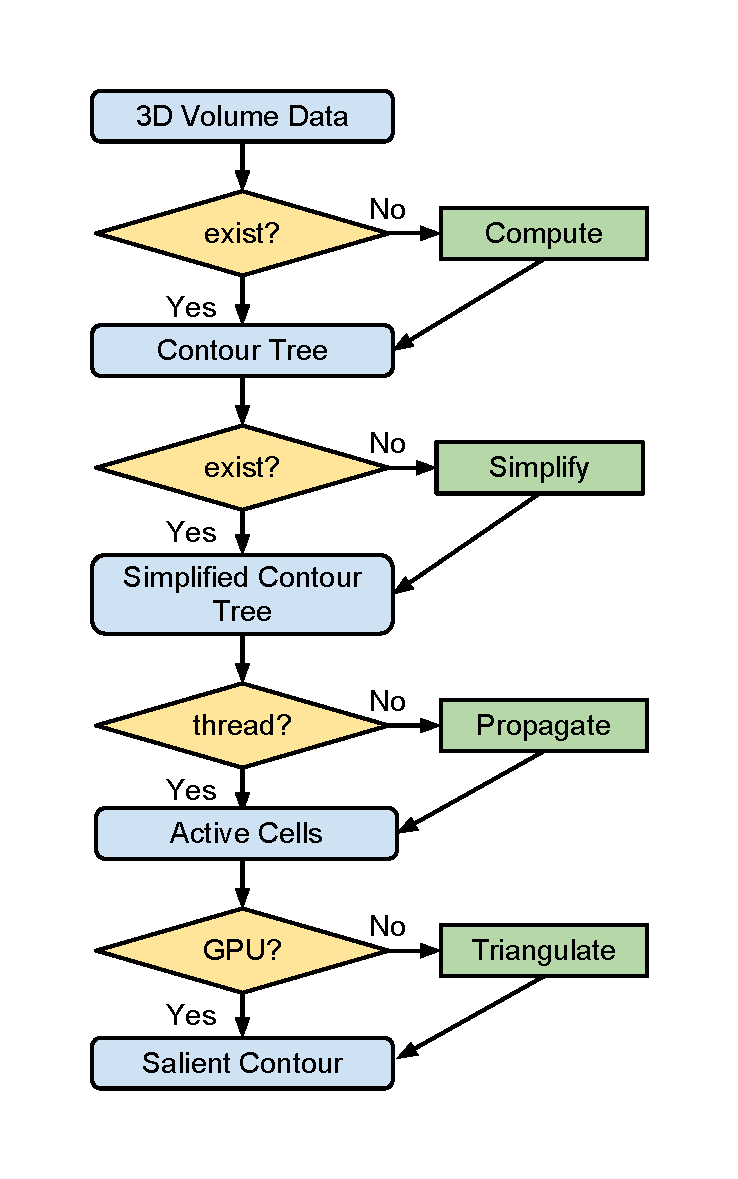
\includegraphics[width=3in]{images/workflow2.pdf}
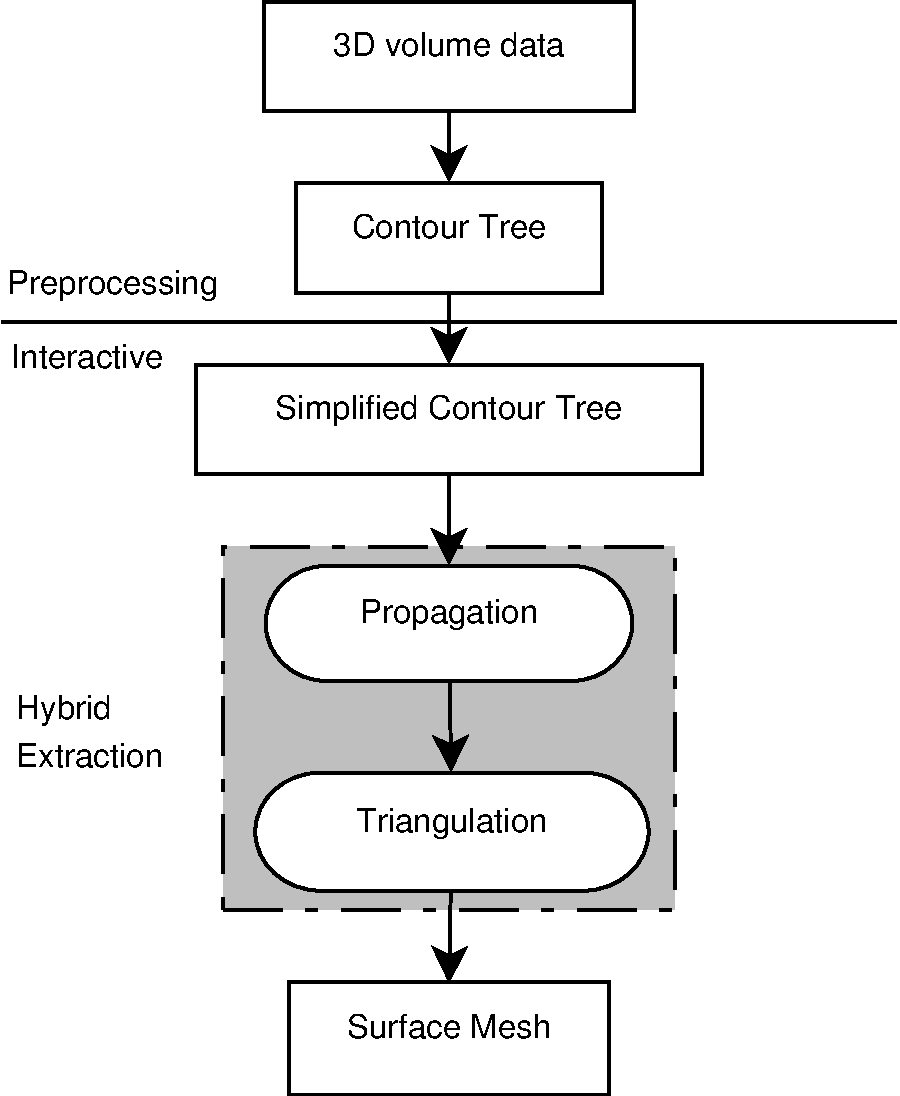
\includegraphics[width=3in]{images/workflow.pdf}
\caption{Overall Workflow}
\label{fig:workflow}
\end{figure}

The rest of the thesis is organized as follows. The method we used for
finding Region of Interest, most of which are previous works, 
are described in Chapter~2% \ref{ch:preworks}
. 
% Some previous works are descripted in Chapter~\ref{ch:related}. 
And then a hybrid accelerated method for propagating the contour and 
triangulating active cells is introduced in Chapter~3 % \ref{ch:prop}
and Chapter~4 
% \ref{ch:interp}
respectively. Chapter~5 % \ref{ch:results}
describes the 
experiment environment and presents the results. 
Finally, a summary of the thesis and the conclusions are drawn in 
Chapter~6 % \ref{ch:conc}
.

%-----------------------------------------------------------------------------
% \include{techintro}
% \chapter{Previous Works}
\chapter*{Chapter 2. ROI Computation}
\addcontentsline{toc}{chapter}{Chapter 2. ROI Computation}
\setcounter{tocdepth}{0}
\setcounter{chapter}{2}
\setcounter{section}{0}
\label{ch:preworks}

This chapter describes the region of interest computation method, most of 
which focused on the preprocessing of 3-dimensional
volume data, which aims to find out the topological structure. 
In our approach, contour tree is used as the abstraction of the 
volume data. Although this won't be
good when the input data is noisy, fast contour extraction method depends
on the generated seed set during preprocessing. And when applied 
simplification methods, it won't be hard to find significant contour 
structures in the original volume.

% The traditional contour propagation method is limited by starting from 
% a single seed and extract the contour by finding neighborhood according 
% to a given isovalue. 

% There are simply two stages in the traditional contour propagation method:
% \begin{itemize}
% \item The goal of the first stage is to ....... This idea is introduce by

% \item But for accerlerating the method, the whole extraction pipeline
% is divided into several stages:
% the parallel
% \end{itemize}
\section{Background Research}

The concept of an ROI, which is a selected subset of samples in a image, 
is commonly used in medical imaging. Typical application covers
the dimension from 2D image to volumetric data and time-varying volumes
and focus on segmenting boundaries in an image or a volume.
% To interactively browse ROI in our application, 

% There already many publications focused on parallel computation of 



\section{Contour Tree}
H. Carr proposed the concept of \emph{flexible isosurface}
\cite{carr2010flexible} and the simplification method to get clean output 
of isosurface mesh. There are several terms defined in this work, such 
as \emph{path seeds} and \emph{local geometric measures} etc.

The local geometric measures can be used to validate individual contours when 
simplifying the contour tree to a hierarchical structure. The basic measure
is to use \emph{topological persistence}, which is the difference in function
value on an edge that connects a pair of critical points. Several other
measures like \emph{surface area} and \emph{integral volume} are used for 
further exploration of the volume.

Contour tree for 3D images is 
introduced by M. Van Kreveld et al.\cite{van1997contour} to improve the speed
of isocontouring. The contour tree is further developed by H. Carr
\cite{carr2000computing} to help the interactive exploration of 
multi-dimensional imaging data.
It is widely used in various field of study, including 
data compression, contour matching\cite{sohn2006time}, GIS etc.
And in various data dimension from 2D images, 3D volume data and 4D 
time-varying volume.

There are various implementations of computing Contour Tree from 2D/3D 
dataset. And among those implementations, H. Carr's method is well-known and 
widely accepted as the general method, which takes $O(N\log N)$ in run-time 
for Contour Tree construction.

\begin{figure}[h!]
  \centering
  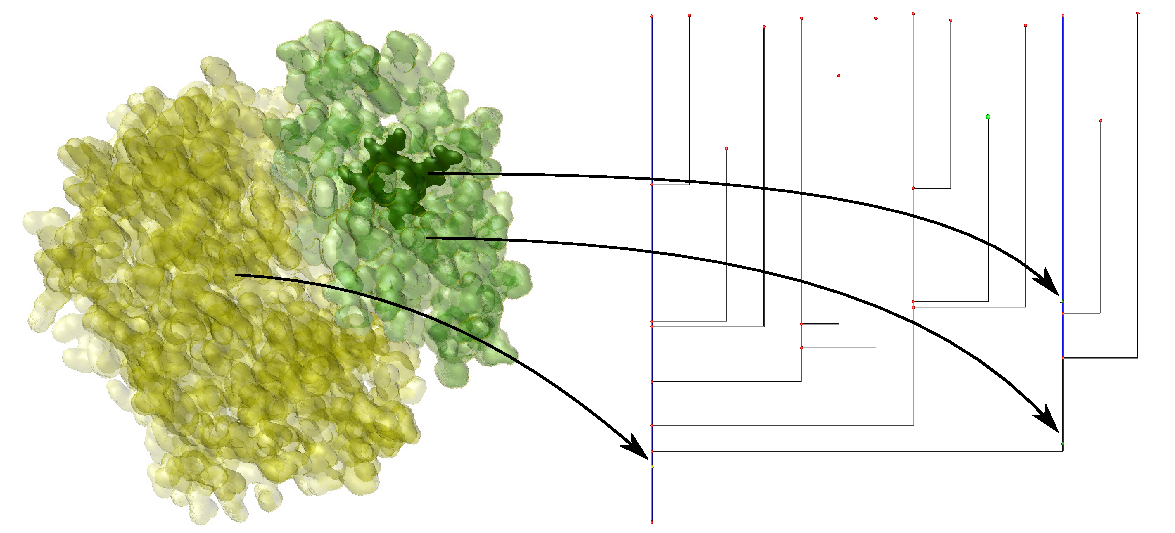
\includegraphics[width=\textwidth-1in]{images/topo-match.pdf}
  \caption{Contour tree mapped to 3D volume data}
  \label{fig:contree-map}
\end{figure}

\subsection{Contour Tree Construction}

To generate the contour tree information, we follow the conventional 
method to create it in $O(n \log n + t\alpha(t))$. We sort the intensity 
values of all voxels in the volume, sweep from high to low isovalues to 
construct join tree using union-find structure\cite{tarjan1975efficiency} 
to determine connected components.

% \begin{figure}[h!]% [htb]
% \centering
% \subfloat[Original Image Input]{\label{fig:blur03}
%   
\includegraphics[width=2in]{images/blur03.png}}
% \subfloat[Join Tree Map]{\label{fig:jtmap}
%   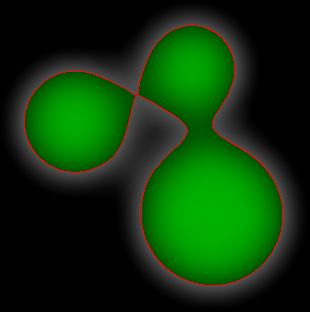
\includegraphics[width=2in]{images/jointreemap.png}}
% \caption{Contour Tree Construction}
% \end{figure}

% In order to illustrate the process of generating the contour tree, a 
% synthesized image (shown in Figure~\ref{fig:blur03}) is created, which is 
% blurred from blobs in a blank image. 

% TODO: describe the method on construting contour tree
The algorithm for computing contour tree described by 
H.~Carr et al.\cite{carr2000computing} consist of the following four steps.
\begin{enumerate}
\enumeratefix{}
\item \textsl{Sort all \emph{n} vertices of the mesh by their intensity values.}
\item \textsl{Perform a sweep of the \emph{n} vertices from lowest values to 
  highest ones to construct \emph{join tree}.}
\item \textsl{Perform another sweep from a reverse direction to construct 
  \emph{split tree}.}
\item \textsl{Merge the join tree and split tree and remove nodes % on the tree
  that keep no topological changes.}
\end{enumerate}

% \subsection{Seed Edge Generation}
To track the individual contour components in the volume data, store edge
information as the seed during the construction of join tree. Then transfer
it to the contour tree during the merge step of the algorithm. 
In the meanwhile, we generate one and only one seed for each contour depend 
on the contour tree information. This provides the information to 
manipulate and annotate individual contours interactively.

In our implementation, the generated seed is stored with contour tree data
file in volume data preprocessing stage. The information can be reused to
generate simplified contour tree interactively as well.

\subsection{Branch Decomposition \& Contour Tree Simplification}
V. Pascucci et al.\cite{pascucci04:_multi} composed a multi-resolution data
structure for representing the contour tree in a hierarchical layout and an 
algorithm to construct it.

\begin{figure}[h!]
  \centering
  \subfloat[coarse simplified 1]{\label{subfig:contree-simp-01}
    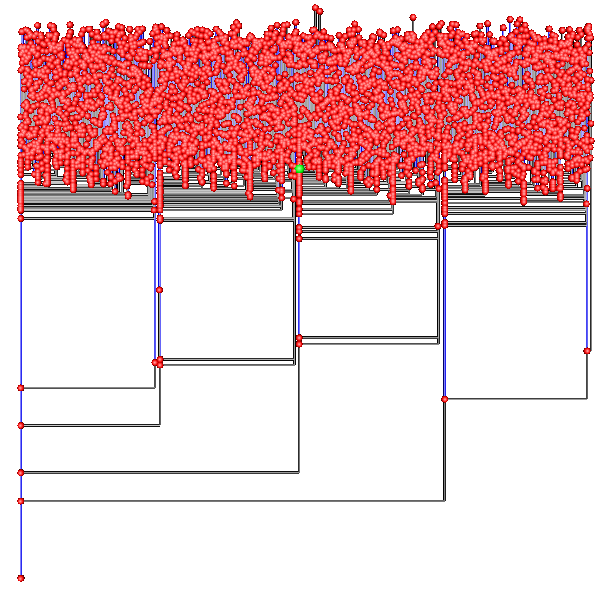
\includegraphics[width=(\textwidth)/3]{images/contree-simp-01.png}}
  \subfloat[coarse simplified 2]{\label{subfig:contree-simp-02}
    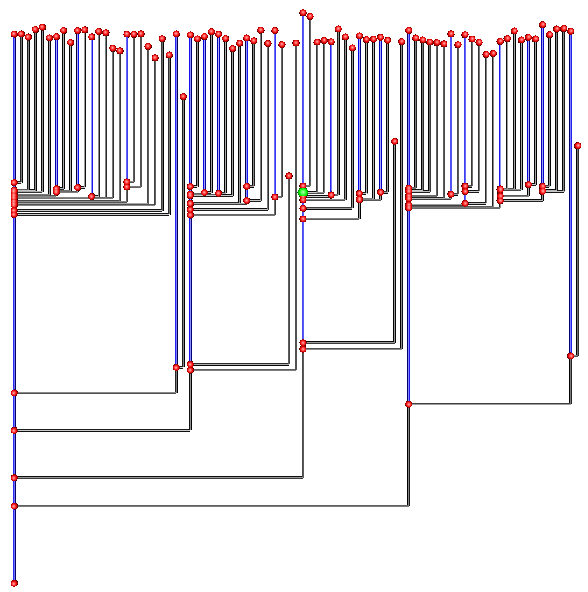
\includegraphics[width=(\textwidth)/3]{images/contree-simp-02.png}}
  \subfloat[fine simplified]{\label{subfig:contree-simp-03}
    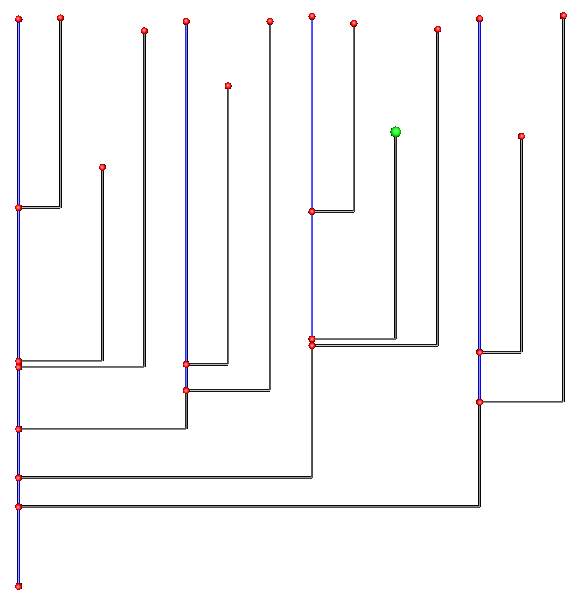
\includegraphics[width=(\textwidth)/3]{images/contree-simp-03.png}}
  \caption{Interactive contour tree simplification}
  \label{fig:contree-simp}
\end{figure}

We implemented the contour tree simplification according to the persistence 
value of each branch, which is the length of the branch. Each saddle-extremum
pair, whose persistence is below a given threshold is considered to be 
insignificant. Therefore, we remove the arc that is consider to be 
unimportant from the contour tree to discard the corresponding noisy 
structures. Besides, we present an interface that can provide threshold
interactively to visualize simplified contour tree.


\section{Contour Property Computation}
C.L. Bajaj et al. \cite{bajaj1997contour} introduced \emph{contour spectrum},
which provides global geometric properties like surface area, volume and
gradient integral of the contour. This work enables the identification
of important isovalues for guiding exploratory visualization through a
simple interface. V. Pascucci et al.~\cite{pascucci2002efficient} propagate 
topological indexes along branches of the contour tree. H. Carr et al.~
\cite{carr2004simplifying} later defined local geometric measures for 
individual contours, such as surface area and contained volume.

\paragraph{Surface Area Computation}

Surface area implies the exposed area of a solid object. For instance, 
surface-area-to-volume ratio(SA:V) of a sphere is small. In the contrary, 
the SA:V ratio of many body parts, say brain, are very large due to 
infoldings, allowing higher rates of metabolism.

We use the additivity property of the surface area add up non-overlap 
triangles of the surface.
$$ A(S) = A(S_1) + \cdots + A(S_r). $$
\paragraph{Gradient Computation}

The gradient of a scalar function $f(x_1, x_2, x_3, \dots, x_n)$ is denoted 
$\nabla f$. The notation $\operatorname{grad}(f)$ is also used for the 
gradient.
$$ \nabla f  = \left(\frac{\partial f}{\partial x_1 },\dots,\frac{\partial f}
{\partial x_n }  \right). $$
In 3-dimensional rectangular coordinates, this can be expanded to
$$\nabla f(x, y, z) = 
\left(\frac{\partial f}{\partial x},
\frac{\partial f}{\partial y},
\frac{\partial f}{\partial z}\right)$$
Therefore, for each triangle $i$, we compute the summation of normal vector 
length and divide it by the area.
% we can compute the gradient value for each triangle by
$$g_i = \frac{|\vec n_1|+|\vec n_2|+|\vec n_3|}{3\times area}$$
And the gradient of the contour component would be the average value of 
those triangles.
$$G = \frac{\sum_{i=1}^n g_i \times a_i}{\sum_{i=1}^n a_i}$$

\paragraph{Volume Computation}
Complex shapes like brain surface can be calculated by 
\emph{integral calculus} in the condition that a formula exists for the 
shape's boundary. Since the procedure of building contour tree sweep
every vertices in the volume and results in contour tree edges which 
represent for monotone structures. The summation of all the cells on 
the monotone structures, which are adjacent to each other on the same 
direction, is the volume corresponding to the contour tree edge. 
This is the information commonly used for estimating whether a contour is 
the region of interest.

%-----------------------------------------------------------------------------
% \include{method}
% \chapter{Related Works}
% \label{ch:related}

% In this chapter, some similiar works are described. A comparison between our
% work with these works are made. This includes the concept of 
% \emph{flexible isosurface}, parallel and out-of-core methods, as well as 
% some GPU-based works.

% \section{Flexible Isosurface}

% % \paragraph{Local geometric measures}
% The local geometric measures can be used to valid individual contours when 
% simplifying the contour tree to a hierarchical structure. The basic measure
% is to use \emph{topological persistence}, which is the difference in function
% value on an edge that connects a pair of critical points. Several other
% measures like \emph{surface area} and \emph{integral volume} are used for 
% different usage.

% \begin{enumerate}
% \item \emph{persistence}
% \item \emph{surface area}
% \item \emph{volume}
% \item \emph{hypervolume}
% \end{enumerate}

% % \paragraph{Contour tree simplification}
% \begin{enumerate}
% \item \emph{leaf pruning}
% \item \emph{vertex reduction}
% \end{enumerate}


%-----------------------------------------------------------------------------
% \include{method}
\chapter*{Chapter 3. Contour Propagation (Multi-core CPU)}
\addcontentsline{toc}{chapter}{Chapter 3. Contour Propagation (Multi-core CPU)}
\setcounter{tocdepth}{0}
\setcounter{chapter}{3}
\setcounter{section}{0}
\label{ch:prop}

In this chapter, we describe a novel algorithm to propagate an individual 
contour from a single seed. The seed is generated during the preprocessing
stage while constructing the contour tree. It is difficult to propagate
a large contour using a parallel method because it's hard to predict the
direction and position the contour. Therefore, we describe our algorithm in
this chapter as the main contribution of the thesis.

% Concurrent queue-based contour propagation method aims to collect active cell
% as well as the compact array for parallel triangulation.

\begin{figure}[htb]
  \centering
  % 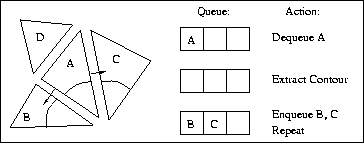
\includegraphics[]{images/img3.png}
  \vspace{20pt}
  \fbox{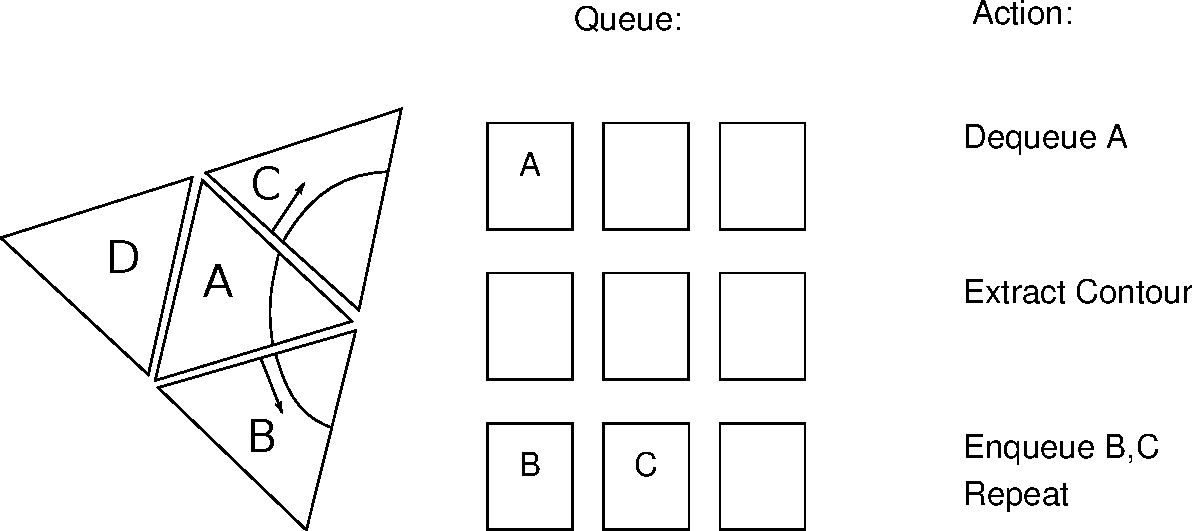
\includegraphics[scale=0.5]{images/drawing3.pdf}}
  \vspace{20pt}
  \caption{Illustration of contour propagation}
  \label{fig:contourpropagation}
\end{figure}
\section{Background Research}

% \subsection{Conventional Contour Propagation Method}

% \subsection{Implementation of Concurrent Queue}

In this thesis, we focus on extract the interactively selected large 
contour component while taking advantage of modern hardware. Conventional
sequential extraction method won't meet our need for real-time interest-base
contour component visualization.

The commonly used method for propagating an individual contour is to compute
the intersected neighboring cell by comparing vertex values with the given 
isovalue. Then push all the intersected neighboring cells into a queue so 
that those cell can be triangulated in later steps. For the case used in 
this thesis, 6 tetrahedrons are divided from a single cube. Therefore, 
the intersected tetrahedron might be a tetrahedron in another cube.

The problem we met to complete the contour propagation in a parallel
way is how to implement the push and pop operations efficient, while 
propagating from a single seed cell to all directions. A naive method that
could be think about is to use a shared queue between all threads while all
operations on the queue should be protected by mutex lock. This could be 
much more efficient than the sequential method due to the reduction of the 
time to compute intersected neighboring cells. Because these operations 
can be done in parallel. However, the time to push and pop in the shared 
queue is not reduced at all. And this could be a major obstacle to improve
the contour propagation.

% Many publications have been focused on the implemenation of a
% thread-safe queue. Since this thesis mainly focus on extracting 3D contour
% start from a given seed cell, 

% \section{A Naive Method}

\section{Concurrent Propagation}
To avoid long time waiting for execution to access shared queue, we designed 
an algorithm to maintain a shared queue and use local queue in each thread,
while use a shared queue to avoid the situation of empty queue starvation.

% touch cell
To prevent duplication when visiting the volume vertices, we maintained a
shared set between all the threads. Since we just store whether the vertex
is visited in the set, the type of is simply a bitset. Although it is shared
between all the threads, it is rarely visited during the propagate progress.
Additionally, the bitset is initialize as 0 and set to 1 when visiting the 
cell. Therefore, it's safe to maintain it as a lock free set.

% shared queue
% the previous work, we put a initial seed cell into the shared 
% queue, then one of the threads aware this initial cell and then start to 
% compare the intensity values of neighboring cells with the given isovalue.

\begin{algorithm}[htb]
  \caption[Parallel propagate function]
  {\emph{propagate} Function\label{alg:propagate}}
  \SetLine
  % \linesnumbered
  \KwIn{Isovalue, Initial Seed Cell, $ThreadID$, Total Number of Threads, 
    Initialized Unvisited Bitset}
  \KwOut{$ActiveCellArray$, Parallel Prefix Sum($Scan$)}
  Create $LocalQueue$\;
  \While{True}{
    $Cell \leftarrow$ \emph{dequeue}()\;
    Get $Vertex$ and $FunctionValue$ of $Cell$\;
    Compute $Index$ by compare($FunctionValue$, $Isovalue$)\;
    $ActiveCellArray[ThreadID]$ $\leftarrow$ $Cell$ and $Index$\;
    \ForEach{intersected adjacent tetrahedron}{
      $AdjacentCell$ $\leftarrow$ GetNeighborCell($Cell$)\;
      \If{$AdjacentCell$ exists \& not visited}{
        Visist($AdjacentCell$)\;
        \emph{enqueue}($AdjacentCell$);
      }
    }
  }
\end{algorithm}

At the starting point of propagation, one of the threads get a seed cell index.
To find intersection points, sampling current cell vertices and function value
and comparing the function value to given isovalue to get intersection 
position. In our case of propagating a tetrahedral mesh, four
sampled values should compare to the isovalue. Then store cell index and 
intersection information into each thread specific active cell array.
This array is later needed as a collection of active cells and its information
to generate parallel prefix sum. Then sample neighboring cells with 
intersection and enqueue it.

% ...

\subsection{Usage of Local Queue}

% local queue
The trick to use local queue in each thread for contour propagation, which 
guarantees no seed loss, mainly focused on how to get a seed. To describe 
Algorithm~\ref{alg:dequeue} the following paragraph gives out a summary of 
the idea:

% \textsl{
To get a cell each time, local queue is visited first. And if there is no 
cell in local queue, the thread will announce that it lack of seed cell for
further propagation, so that other threads might aware this and push a cell 
into the shared queue. Then go on to check out whether all the other local
queues are empty. Now that all the local queues and shared queue are empty,
it means that all the propagation progress is finished and the instance
of current thread should be terminated. But if the local queue in one of the 
other threads is not empty, the current thread will go on to the next loop
to find out whether a seed cell is pushed into the shared queue.
% }

\begin{algorithm}[htb]
  \caption[Dequeue function]{\emph{dequeue} Function\label{alg:dequeue}}
  \SetLine
  % \linesnumbered
  % \KwIn{$Isovale$, $SeedCell$, $ThreadID$, $NumberOfThreads$}
  % \KwOut{Cell}
  \eIf{$LocalQueue$ is not empty}{
    $Cell$ $\leftarrow$ Pop($LocalQueue$ front element)\;
  }{
    \While{True}{
      LackOfSeedFlags[$ThreadID$]$\leftarrow$ True\;
      \eIf{$Cell \leftarrow$Dequeue($SharedQueue$) failed
        \label{code:dequeue}}{
        \eIf{all LackOfSeedFlags is False}{
          TerminateThread($ThreadID$)\;
        }{
          % Find Cell in $SharedQueue$\;
          \textbf{continue};
        }
      }{
        LackOfSeedFlags[$ThreadID$]$\leftarrow$ False\;
        \textbf{break};
      }
    }
  }
\end{algorithm}

% dequeue
On Line~\ref{code:dequeue} of Algorithm~\ref{alg:dequeue}, we check the size of
shared queue and then dequeue it immediately after the check in the same 
function with lock protection. Otherwise, it can't guarantee there is element
while dequeue it from shared queue, because the instance of shared queue might
be different between the time when check the size of the queue and dequeue
function is called.

\begin{algorithm}[htb]
  \caption[Enqueue function]{\emph{enqueue} Function\label{alg:enqueue}}
  \SetLine
  % \linesnumbered
  % \KwIn{$LackOfSeedFlags$, $LocalQueue$, $SharedQueue$, $AdjacentCell$}
  % \KwOut{Cell}
  \eIf{all $LackOfSeedFlags$ is False}{
    $LocalQueue \leftarrow$ Push($AdjacentCell$)\;
  }{
    $SharedQueue \leftarrow$ Push($AdjacentCell$)\;
  }
\end{algorithm}

Consequently, when propagating with a seed cell, the neighboring cells will 
be pushed into local queue if all other threads didn't make the lack of seed
announcement. Otherwise, the new generated seed should be pushed into the
shared queue to meet the needs of local queue(s) of other threads.

\subsection{Post-processing}

For each active tetrahedral cell in active cell array, there might be one or
two corresponding triangles, which depends on the intersection position on the
tetrahedron. To finish this step in an efficient way, a simple CUDA kernel was 
made to generate the array for generating mesh in parallel pipeline while 
avoiding conflicts between CUDA threads.

\begin{table}[htb]
  \centering
  \begin{tabular}{p{\textwidth/2}|p{\textwidth/2}}
    \hline
    \multicolumn{1}{c}{Sequential} & \multicolumn{1}{c}{Parallel} \\
    \hline
    \texttt{\textbf{for} \textit{j} from 1 to n \textbf{do}} & 
    \texttt{\textbf{foreach} \textit{j} in parallel \textbf{do}} \\
    \hspace{10pt} \texttt{scan[\textit{j}] = scan[\textit{j}-1] + f(in[\textit{j}-1]);} & 
    \hspace{10pt} \texttt{scan[\textit{j}] = f(in[\textit{j}]);} \\
    \hline
  \end{tabular}
  \caption{Comparison of sequential and parallel \emph{scan} generation}
  \label{tab:scan}
\end{table}

By comparing given isovalue with intensity values of neighboring cell to get the 
intersected neighbors next to it, we can get the parallel prefix sum 
\cite{harris2007parallel} of each active voxel.
\footnote{http://http.developer.nvidia.com/GPUGems3/gpugems3\_ch39.html} 
This can be used for predicting the size of output triangles in CUDA memory.

% There are several implementation tricks that worth to state:
% \begin{itemize}
% \item During generating active seed array, it should be allocated as a normal
% instead of using \textsf{vector} in STL. This can prevent an inefficient copy
% of the array to allocate it and copy it to GPU.
% \item 
% \end{itemize}

% \begin{figure}[h!]
%   \centering
%   % 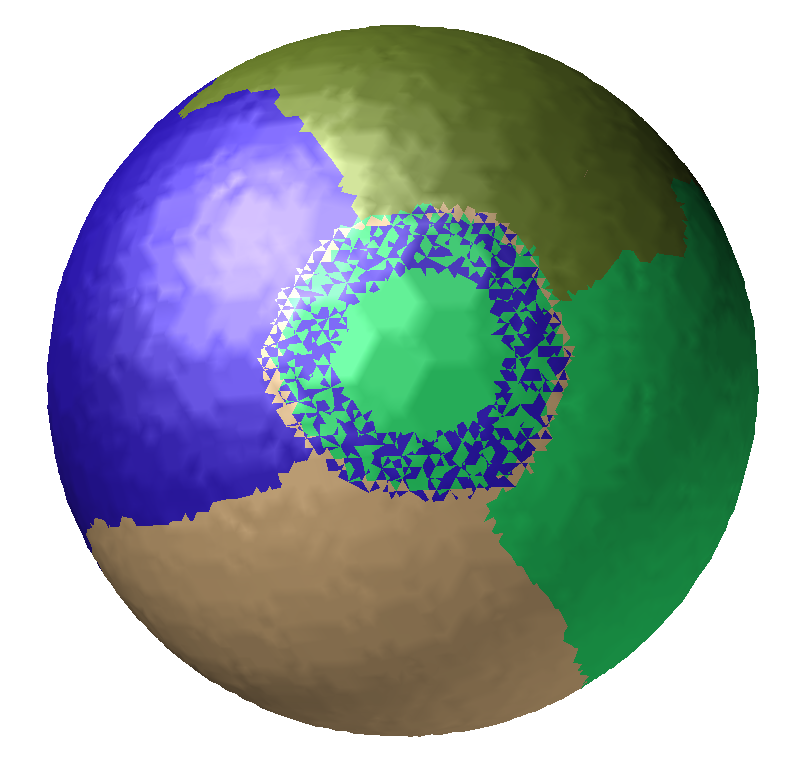
\includegraphics[width=\textwidth/3]{images/mt-sphere-propagate}
%   \fbox{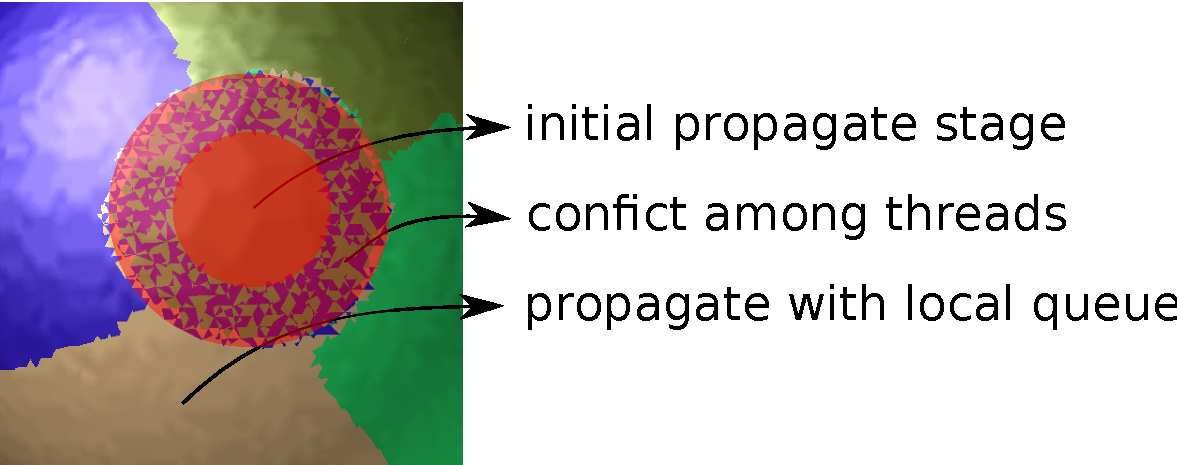
\includegraphics[width=\textwidth-1in]{images/mt-sphere-crop-intro}}
%   \caption[A typical model of contour propagation in parallel]
%   {A typical model of contour propagation in parallel from the an 
%     initial seed cell (color-tags showing contribution of different threads)}
%   \label{fig:mt-sphere-propagate}
% \end{figure} 

%-----------------------------------------------------------------------------
% \include{method}
% \chapter{GPU-based Triangulation}
\chapter*{Chapter 4. Active Cell Triangulation (Many-core GPU)}
\addcontentsline{toc}{chapter}{Chapter 4. Active Cell Triangulation (Many-core GPU)}
\setcounter{tocdepth}{0}
\setcounter{chapter}{4}
\setcounter{section}{0}
\label{ch:interp}

Due to the parallel architecture on modern graphics cards, a mount of 
graphics related as well as general purpose applications are developed on top 
of GPU. Those applications might be implemented in shader languages like GLSL 
or general purpose computing languages like OpenCL. And among those 
implementations, NVIDIA's CUDA architecture is widely used due to the highly
optimized CUDA libraries and regularly updated SDK. Even many of the modern
supercomputers consist of thousands of NVIDIA's GPUs.

\begin{figure}[H]
  \centering
  \fbox{
    \subfloat[wireframe of active cells]{
      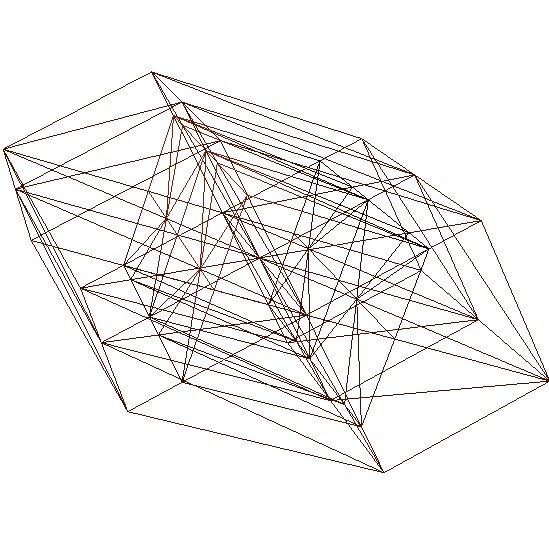
\includegraphics[width=(\textwidth-2in)/2]
      {images/triangulate-cubes2-1.png}}
    \subfloat[shaded mesh]{
      
\includegraphics[width=(\textwidth-2in)/2]
      {images/triangulate-cubes2-2.png}}
  }
  \caption[Cell triangulation]{Cell triangulation 
    (only tetrahedral cells with intersection is triangulated in GPU)}
  \label{fig:cell-tri}
\end{figure}

\section{Background Research}

% Focus on gpu-computing models

% Histopyramid-based method \cite{dyken2008high}

% \subsubsection{Geometry Shader Programming Model}
% Geometry shader based active cell triangulation 

For triangulate active cells extracted from a initial seed cell using geometric
propagation method, GPU implementation is a decent choice to consider. C. Dyken
et al.\cite{dyken2008high} composed a method to enable MC algorithm running
on GPU using shader programming while taking the advantages of a data packing
structure called \emph{HistoPyramids}. 

\begin{figure}[htb]
  \centering
  % 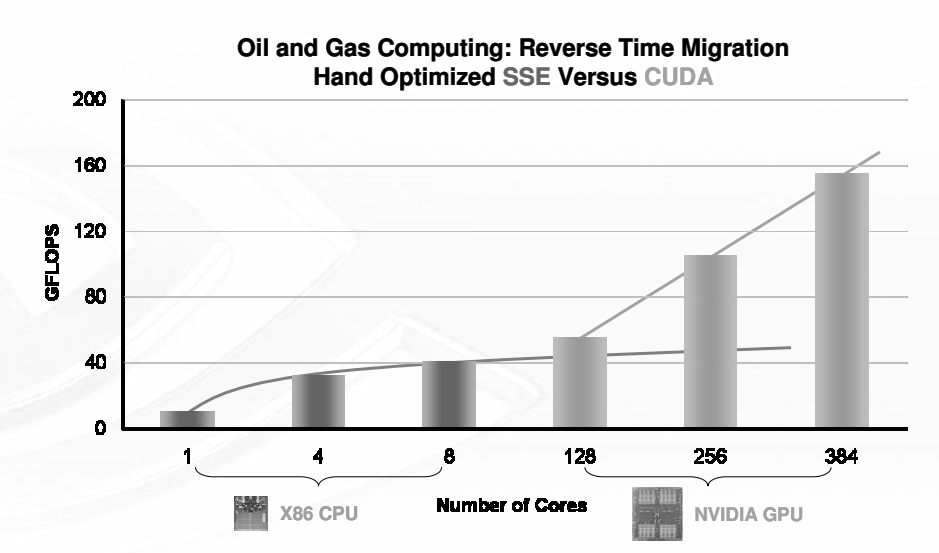
\includegraphics[width=5in]{images/cuda-linear-scaling2.png}
  \fbox{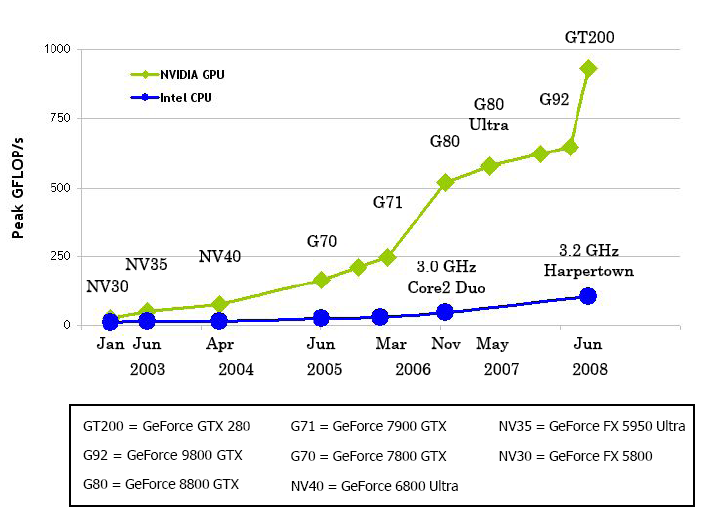
\includegraphics[width=\textwidth-2in]{images/gpu_vs_cpu}}
  \caption{Difference between CPU and GPU in parallel computing}
  \label{fig:cudaintro}
\end{figure}

% Although recent developed GPUs are highly optimized for performing geometry
% operations. But for triangulating active cell, we ...

Vertex shader based active cell triangulation \cite{goetz2005real} focus
on the technique to pack the active cell data to compact them as small as
possible to improve the transfer speed. And even intensive values can be
transferred to GPU during the rendering process. It's good to render dataset
that is large in volume, due to the algorithm don't require a initialize
step to put all volume to GPU as texture.

All of these implementation got a common problem on copying GPU precomputed 
mesh into main memory to prevent duplicated computations. That is to said 
it will triangulate active cells even when operations like rotation was 
made. It cost much unnecessary GPU computation when using shader programs 
for triangulation. 

% advantage

% limitation
In general, shader-based triangulation method is much easier to implement,
but far less efficient comparing to the general-purpose GPU programming 
methods due to the difference of graphics programming implementation. 
Therefore, it's the limitation of the shader programming method for 
extracting isosurface\cite{goetz2005real}.

% \subsubsection{CUDA Programming Model}

The following is a comparison between the three widely used GPU programming 
APIs:
\begin{itemize}
\item \textbf{OpenCL}: Khronos Group's OpenCL cross-platform and implemented 
on both Nvidia and AMD's GPUs. It can be easily ported to multi-core 
exections. However, it is less developed comparing to CUDA.
\item \textbf{CUDA}: Nvidia's CUDA is currently most highly developed GPU 
programming architecture. It features in various GPU memory management and 
graphics related interoperability. However, it is only available on 
Nvidia's graphics cards.
\item \textbf{DirectCompute}: DirectX compatibility, but limited to Microsoft 
Windows 7 and Vista.
\end{itemize}

Advantage of GPGPU programming : save proceeded data into memory and use 
synchronize method to guarantee to correctness of computing and improve the 
speed further.

% \subsubsection{Vertex Buffer Object}

Faster large object rendering method for preventing overhead of calling
data input functions.

% \subsection{Geometry Shader Programming Model}

% % advantage

% % limitation
% The limitation of the shader programming method for extracting isosurface.
% \cite{goetz2005real}

% \subsection{CUDA Programming Model}

% advantage of GPGPU programming : save proceeded data into memory.

% \subsection{Vertex Buffer Object} 

% faster large object rendering method for preventing overhead of calling
% data input functions.

\subsection{Parallel Contour Extraction Methods}
C.L. Bajaj et al.\cite{bajaj1999parallel} designed out-of-core algorithm aim
to extract huge dataset using a parallel method. Depending on the static 
analysis information precomputed, the algorithm focused on loading balance 
and minimize secondary memory access. A volumetric dataset is divided into 
the atomic processing elements called \emph{blocklet}. Therefore, only cells 
intersected with a range of isovalue would be loaded into main memory.
This approach efficiently reduced the data loading to avoid visiting blocklets
that don't contain active cells. Similar work was done to the GPU 
processing method. Goetz et al.\cite{goetz2005real} developed the method to
carefully compact active cell data as texture and extract the surface
using vertex shader. The algorithm aim to reduce the data transaction 
by concatenate the vertex data with a bitwise operation, so that small portions
in large volume data can be visualized with GPU acceleration. However, the
performance of this work mainly depend on the speed of data transaction to
the graphics card. 

\subsection{Parallelism in CUDA Infrastructure}
Note that an implementation of the Marching Cubes method 
\cite{nvidia:_march_cubes_isosur} exist in recent version of CUDA SDK. This 
program takes the advantage of the parallel structure of CUDA to extract all 
of the cells in the given volume data. % A typical result is shown in Figure~
% \ref{fig:_cuda_mc}. 
Although it's fast enough to extract 
large volume data in real-time, but obviously it won't be possible for this 
program to process datasets as huge as Giga Bytes. Consequently, active cells 
that are needed to be triangulated should be preprocessed before loading the 
whole volume data into CUDA memory. A detail solution is given in Chapter~
4% \ref{ch:interp}
.

\begin{figure}[h!]
  \centering
  % 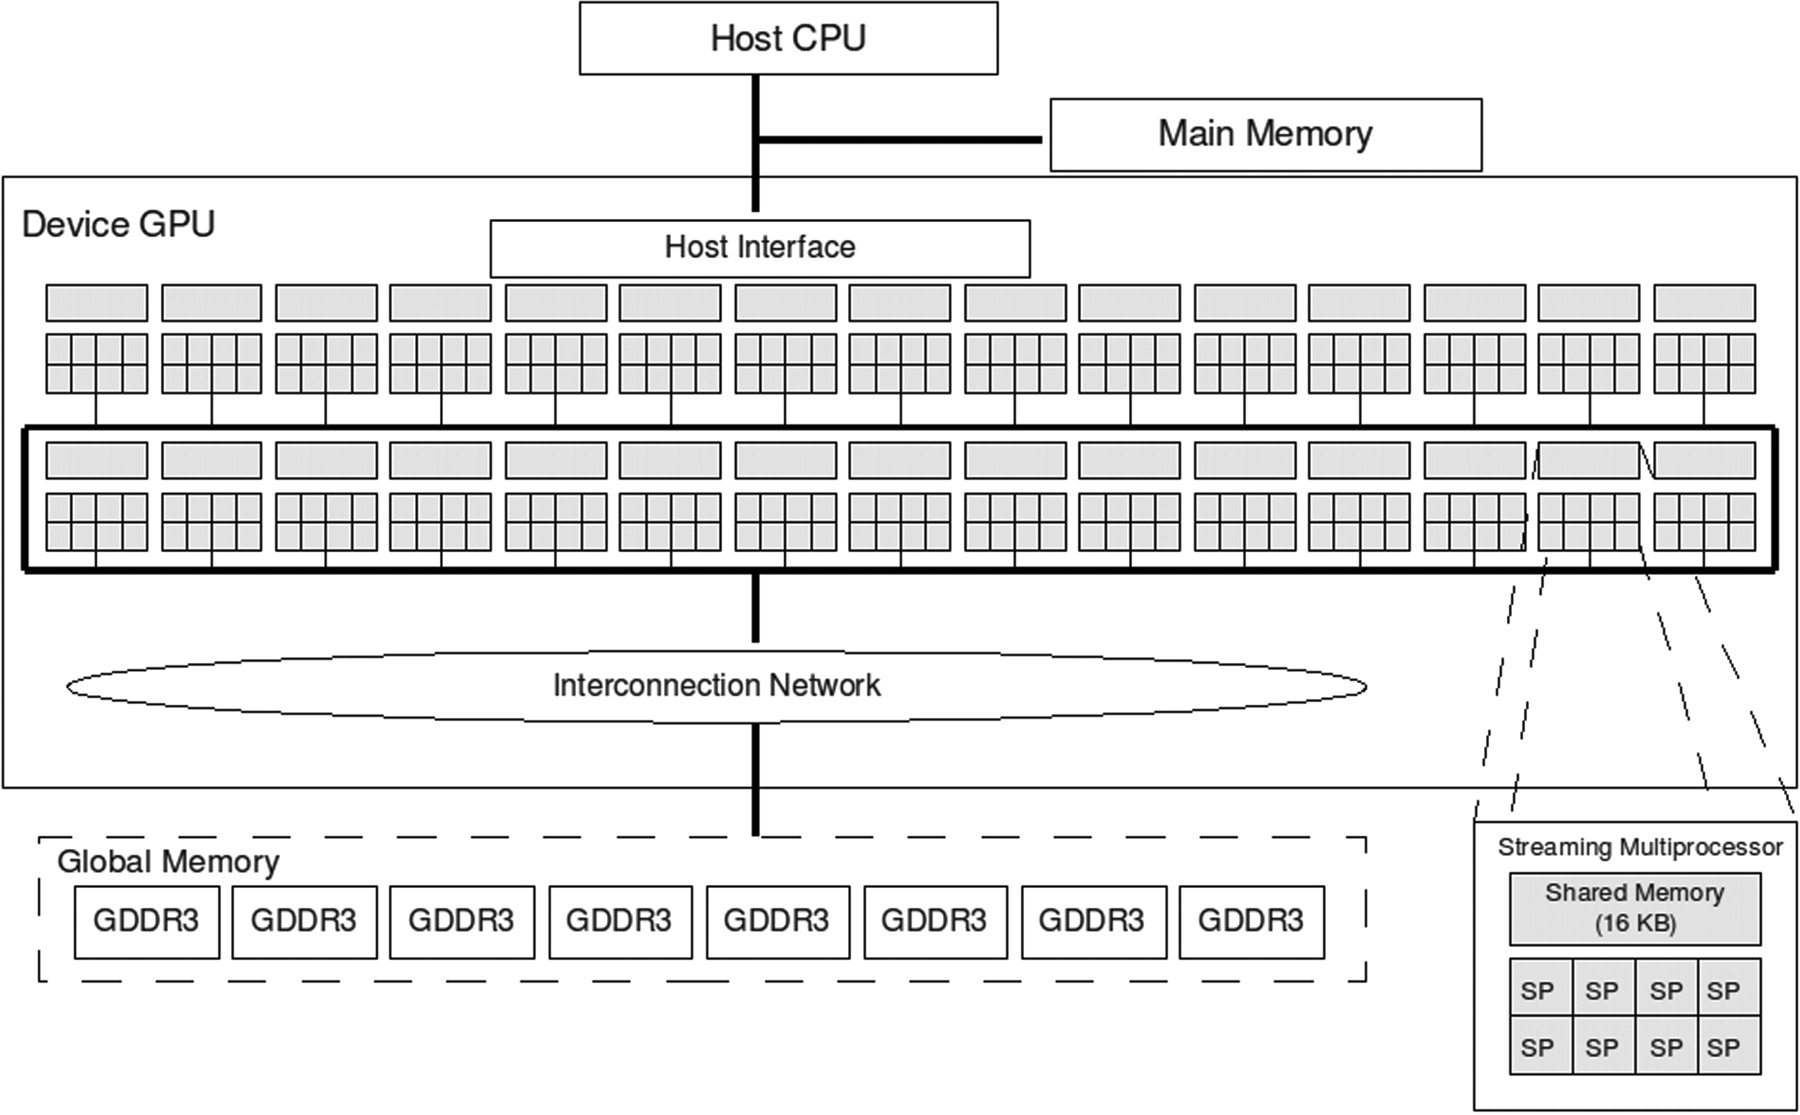
\includegraphics[width=\textwidth]{images/cudaintro.jpg}
  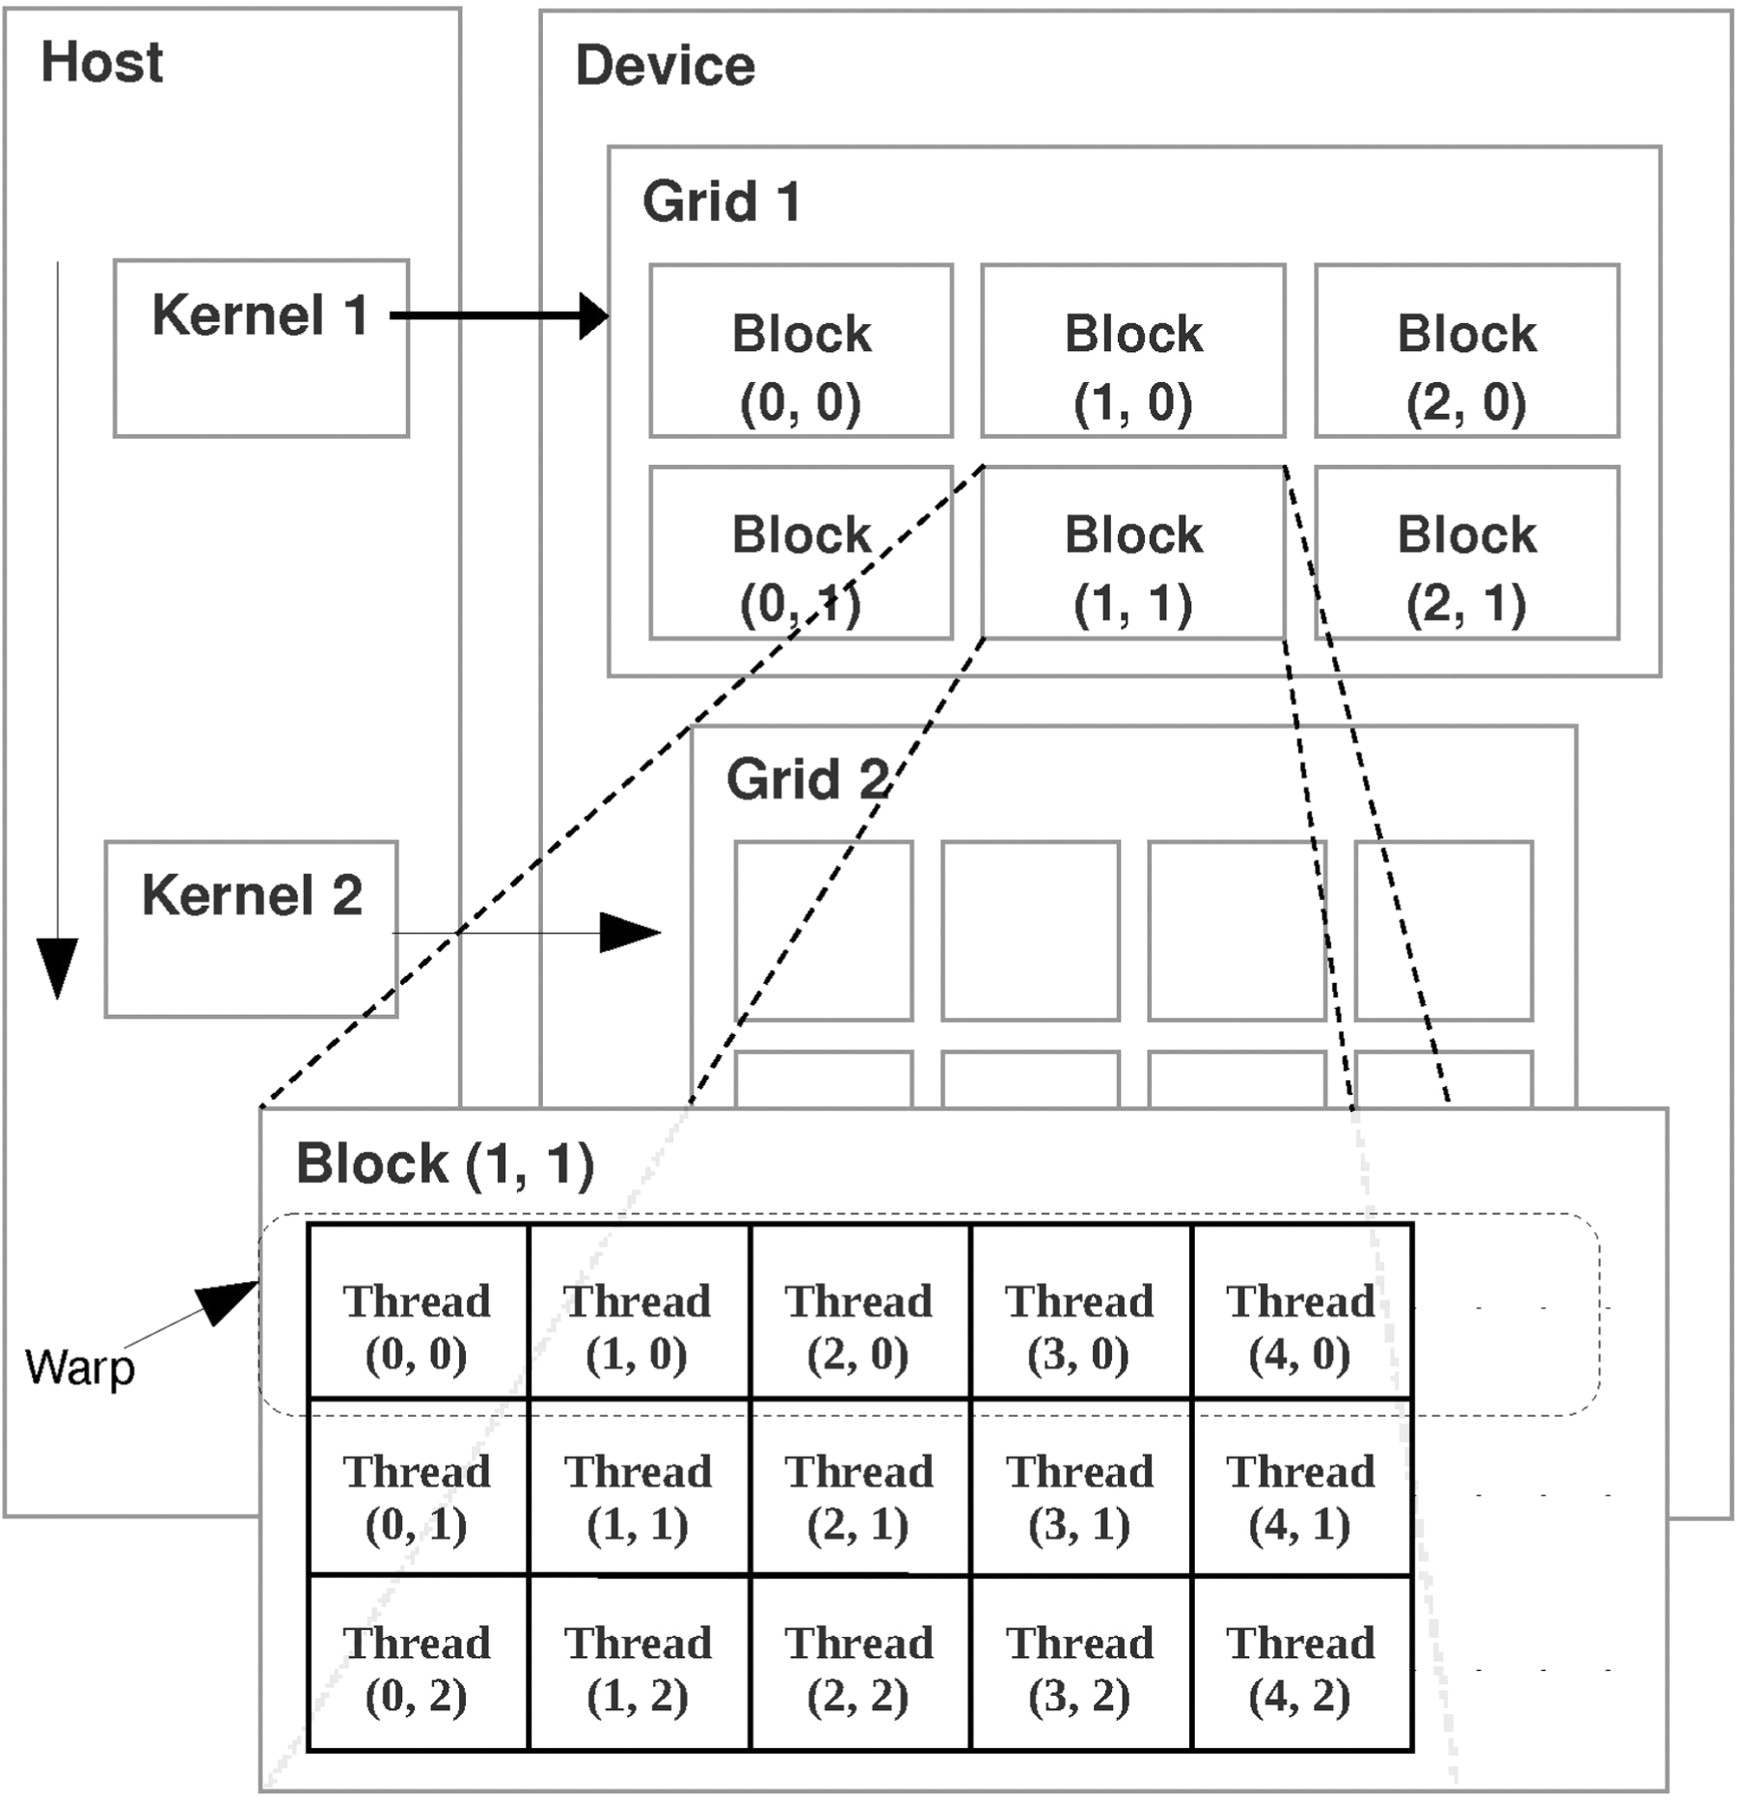
\includegraphics[width=\textwidth-1in]{images/executionmodel.jpg}
  % \includegraphics[width=\textwidth-2in]{images/drawing3.svg}
  % 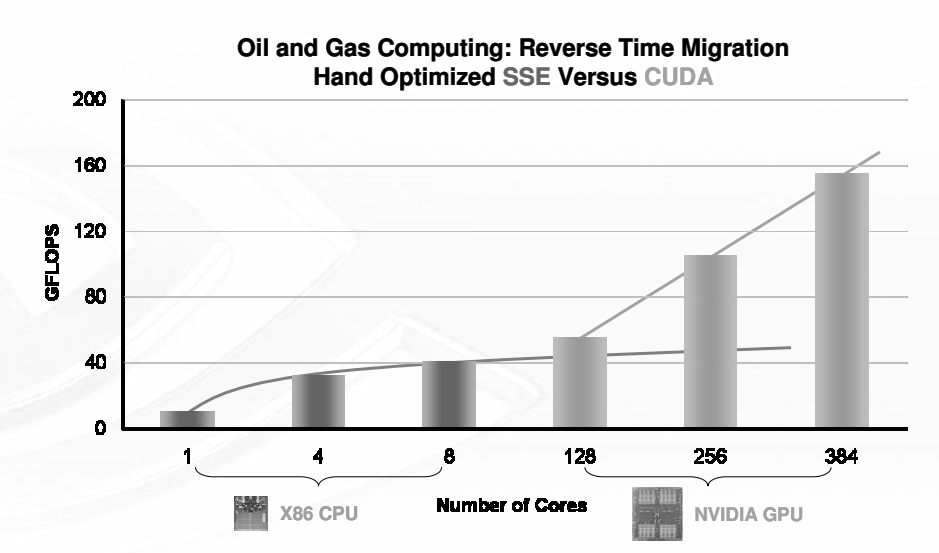
\includegraphics[width=5in]{images/cuda-linear-scaling2.png}
  \caption{CUDA Execution Model}
  % \caption{Linear Scaling with Multiple GPUs}
  \label{fig:_cuda_exec}
\end{figure}

Figure~\ref{fig:_cuda_exec} illustrates the relationship between host and
graphics device. The computing units on each graphics card are divided into
several grids, and each grid consists of a number of blocks, where many 
threads could be run in parallel. And the execution is enabled to 
assign the work to each block, therefore, it's efficient to use CUDA for 
the computation of large amount of simple works.
 
% \subsection{Marching Cubes CUDA Implemenation}

% \begin{figure}[H]
%   \centering
%   \includegraphics[width=3in]{images/SDKSampleMarchingCubes}
%   \caption{CUDA Marching Cubes}
%   \label{fig:_cuda_mc}
% \end{figure}

% \section{Active Cell Decomposition}

\section{Active Cell Triangulation}

Right after the active cell array is computed, a GPU array can be allocated
same size of the active cell array, where consist of the continuous indices 
of tetrahedron intersected with given isovalue.


% volume data allocation
Note that in order to triangulate the volume data that is larger than GPU 
memory, volume data can be allocated and compacted after active cell array
computation instead of loading the whole volume. However, this would slow 
down the triangulation time and might be slower than CPU depending on the
size of the chosen contour.

% OpenGL interoperability
Taking the advantage of CUDA's interoperability with OpenGL\footnote{In 
fact, Direct3D interoperability is also available. In our implementation, 
to enable the program both in Win32 and Linux, OpenGL functions are used.},
vertex buffer object(VBO) is mapped into the address space of CUDA before
launching triangulation computation kernel. And right after the CUDA 
triangulation, buffer object is unmapped from device memory address.
\footnote{Note that a buffer object must be registered to CUDA before it
can be mapped. This is done with \texttt{cudaGLRegisterBufferObject} 
function.}

% index maintain and load tables as texture
There are three tables that can be loaded as texture\footnote{However, for 
tables that are small in size, it's good to put it directed into device 
memory for high speed of access during execution.}. One is the triangle 
table that maps same tetrahedron vertex index to a list of up to 2 
triangles which are built from interpolated edge vertices. And in the
case of triangulation on a single cube, there would be up to 5 triangles.
The reason cubic data in the volume are divided into tetrahedron is 
mainly because of the ambiguity problem when building the contour tree.
Dividing the cube avoids the ambiguity problem and guarantees the 
topology equivalent property between the contour tree and volume data.
Two other tables are an edge table which is used for mapping vertices to edges
that are intersected and a cube dividing table which is used for storing
tetrahedron connectivity information in a cube.

The most difficult problem to the triangulation tetrahedron cell is how
to organize vertex index and and put interpolated information into 
global memory without conflict. To solve this problem, cell intersection
on edges are estimated after combining active cell in CPU.

% ... \& ...
% (... two other tables that are build as texture ... and how/why they are
% used during triangulation in GPU.)
% (... argu about the efficiency on the method ...like the reason to compute
% \textit{code} again instead of copying it from precomputed \textit{code} in
% CPU.)

% parallel prefix sum
With compact array (parallel prefix sum), we perform linear interpolation on
each intersect edge of all active cells. 

% \subsection{Surface Geometric Property Computation}
% The computation of surface area and surface gradient is completed in 
% CUDA kernel execution.

\begin{figure}[H]
  \centering
  \fbox{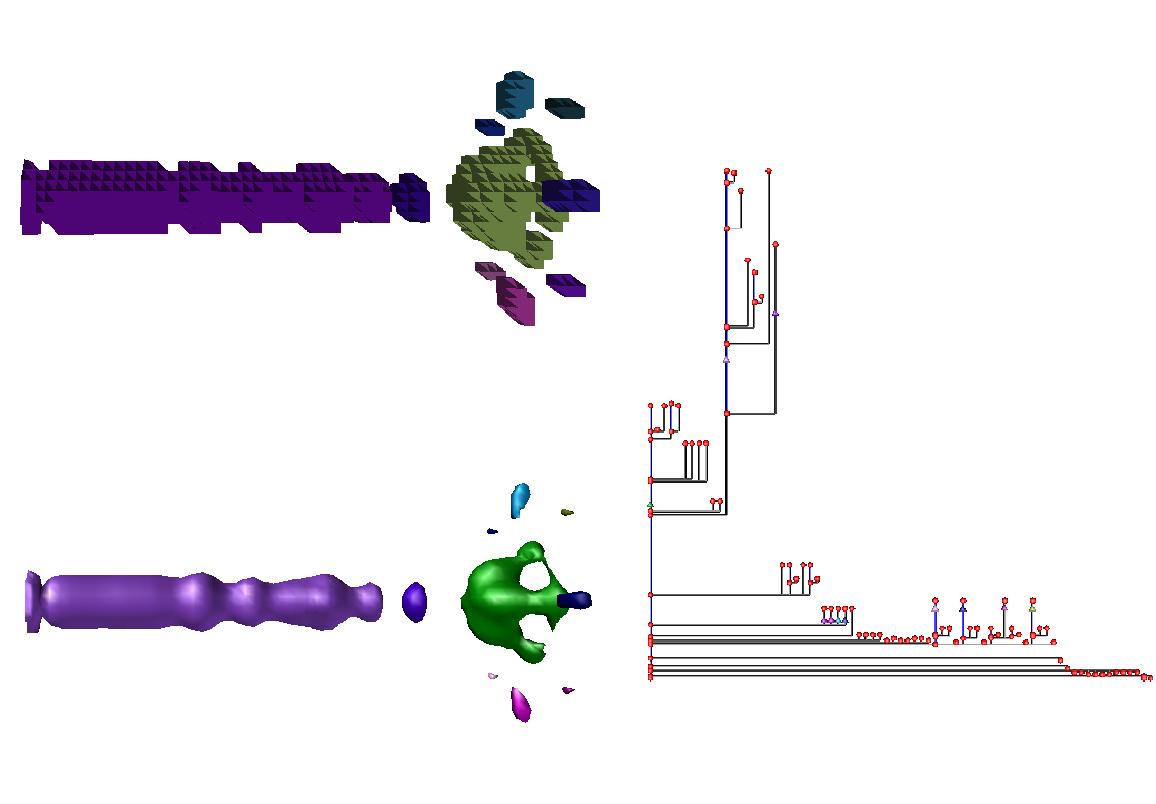
\includegraphics[width=\textwidth-1in]{images/activecell-fuel.pdf}}
  \caption[Collection of active cells are copied to GPU for triangulation]
  {Only cell blocks with intersection are copied to GPU for triangulation, this
    improved the efficiency by avoid visiting empty cells.}
  \label{fig:actcell-tri}
\end{figure}

% \paragraph{surface normal}
For Surface smoothing, surface normal is computed during the triangulation 
process. In our implementation, we use Gouraud shading method for balance the
fast processing and rendering quality. The computation of Gouraud shading
produces continuous shading of surfaces by estimating surface normal of each
vertex in the polygonal 3D model. The normal on each vertex are set to be
the average value of all neighboring vertices.

% \paragraph{surface gradient}

% \paragraph{surface area}


\section{VBO-based Rendering}

There are several reasons to apply VBO rendering to the implementation:
First, it is a time-consuming task to cost memory data from GPU to main 
memory. Second, \texttt{glVertex*} has the potential to be slower, because
there is more call overhead than \texttt{glDrawElements}.
Further more, it's duplicate data transfer between main memory and GPU.

% Rendering performance has at least 4 potential bottlenecks. Unfortunately performance issues often are an interaction of several of them.
% 1) The speed at which data can be moved from the application to OpenGL. (like glVertex, vertex arrays, downloading textures, etc)
% 2) The speed at which data can be moved from OpenGL to the graphics card (DMA or fast-writes over the AGP bus)
% 3) The speed at which geometry transformation, lighting, clipping, vertex shader programs etc can be done.
% 4) The speed at which rasterization, (texture mapping, are you texture memory limited? z-buffering, fragment shading etc etc) can be done.

Due to the usage of parallel prefix sum in our method, the GPU memory to put
all triangles are allocated as vertex buffer object(commonly known as VBO) 
immediately after the current propagation stage. This section of global memory
in GPU is then filled with triangulated mesh data during GPU-based 
triangulation. VBO is used to reduce of avoid large amount of function calling
while rendering triangulated mesh and reduce data transfer from between GPU
and CPU.
% Store triangulated mesh into memory and render it ..




%-----------------------------------------------------------------------------
% \include{results}
\chapter*{Chapter 5. Results}
\addcontentsline{toc}{chapter}{Chapter 5. Results}
\setcounter{tocdepth}{0}
\setcounter{chapter}{5}
\setcounter{section}{0}
\label{ch:results}

In our tests, we use a Linux system (Debian 6.0 Distribution) equipped with 
a hexa-core processor (AMD Phenom II X6 1055T) running at 3.30 GHz, 8GB RAM, 
as well as Nvidia GeForce GTX 460. The graphics card is enabled with CUDA 
compute capability 2.1. 
The graphics card specific CUDA compute capability table are available on 
the Nvidia's official site\footnote{http://developer.nvidia.com/cuda-gpus}.
Tested datasets are vary from molecule data to large scan medical image 
volume data, many of which were provided on \textsl{http://www.volvis.org}.

\begin{figure}[h!]
  \centering
  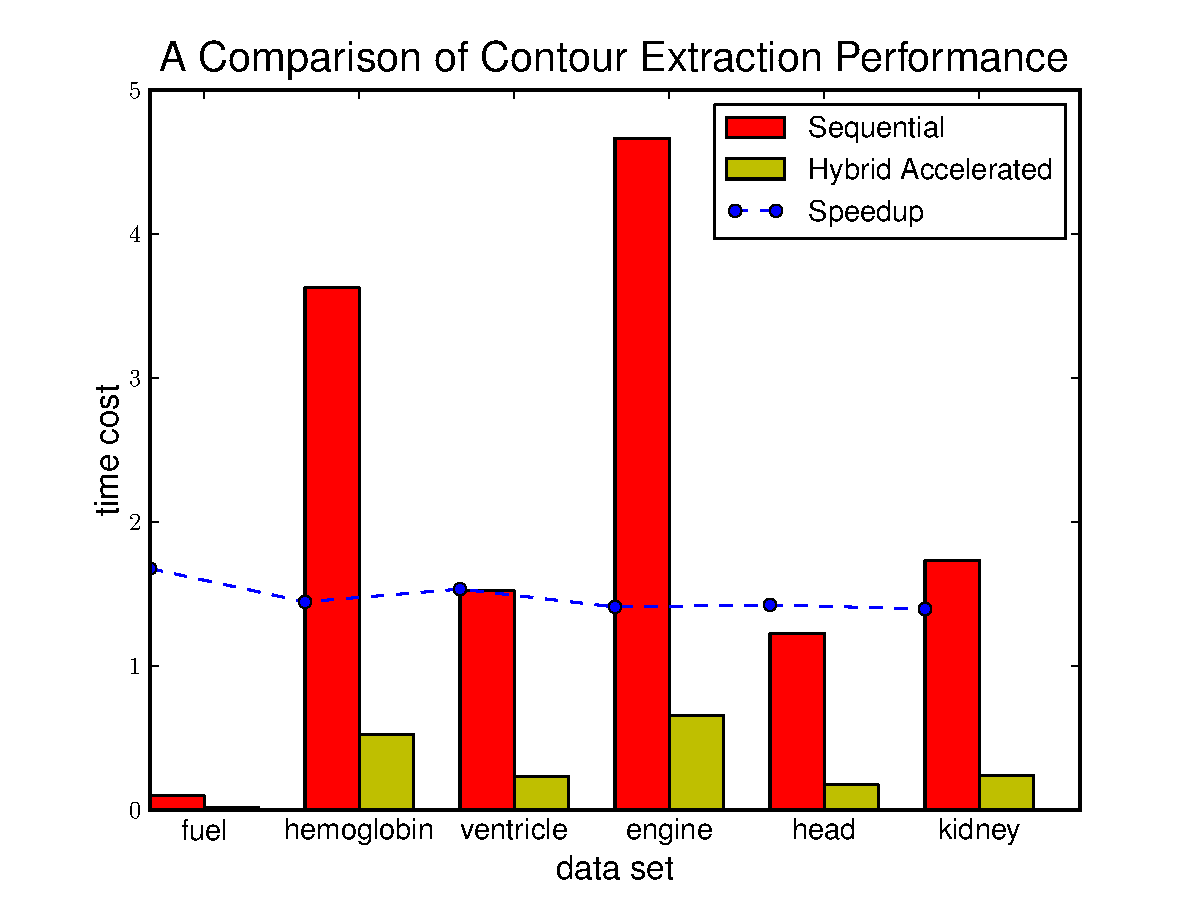
\includegraphics[width=\textwidth-1cm]{images/fig-perf-bar.pdf}
  \caption[Performance comparison with the original method]
  {A performance comparison between conventional sequential program and the 
    composed hybrid accelerated method. (A stable speed improvement up to 
    6$\sim$7 times is shown in blue curve)
    % (executed on Linux environment with AMD Phaand Nvidia
    % GeForce GTX 460 graphics card)
  }
  \label{fig:_perf_bar}
\end{figure}

% \clearpage{}

% \begin{figure}[h!]
%   \centering
%   \subfloat{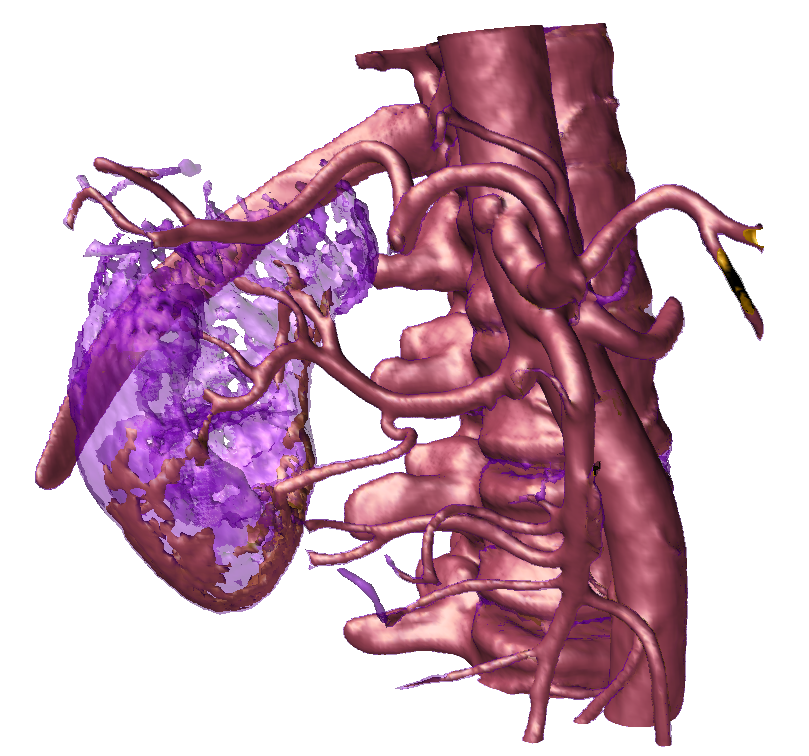
\includegraphics[width=\textwidth-3in]{images/cta_kidney}}
%   \caption[Region of interest in scaned kidney data]
%   {Surface of kidney is clearly shown with support of alpha blending, while noisy 
%     structures are significantly removed.}
%   \label{fig:cta_kidney}
% \end{figure}

% \begin{table}[h]
%   \centering
%   \begin{tabular}{|c|c|c|}
%     \hline
%     Model & Version & Feature \\
%     \hline
%     mostly G8x and G9x & 1.0 or 1.1 & atomic in global memory etc.\\
%     \hline
%     mostly GTX 200 Series & 1.2 or 1.3 & atomic in shared memory etc.\\
%     \hline
%     mostly GTX 400 Series & 2.0+ & threads block etc.\\
%     \hline
%   \end{tabular}
%   \caption{CUDA compute capability}
%   \label{tab:cuda_comp_}
% \end{table}

In this thesis, a comparison on performance is made between conventional 
approach and the composed new method. The results largely depend
on the hard limitations such as bandwidth between CPU and GPU,
the number of cores exists in CPU and GPU. However, on most modern 
computers equipped with Nvidia's GPU, relevant fast contour visualization
is achieved as is shown in Figure~\ref{fig:_perf_bar}.

% \clearpage{}
\section{Propagation Performance}
Here we make a comparison between our proposed results with original 
sequential method. It's not hard to find out the speed improvement from 
Table~\ref{tab:cpuperformance}. The performance highly depends on the usage 
of threads, but too many thread usage will lead to overhead global queue 
usage. Consequently, the number of threads is usually configured as many as 
the number of cores in the CPU to get best performance on the computer.

% \begin{figure}[htb]
%   \centering
%   \includegraphics[width=3in]{images/mt-hbmatch-1.png}
%   \caption{Whole Hemoglobin}
%   \label{fig:hbmatch-1}
% \end{figure}

% \begin{figure}[htb]
%   \centering
%   \includegraphics[width=2in]{images/mt-hbmatch-3.png}
%   \caption{Hemoglobin Portion}
%   \label{fig:hbmatch-3}
% \end{figure}

\begin{figure}[htb]
  \centering
  \subfloat[front]{
    \label{fig:engine-1}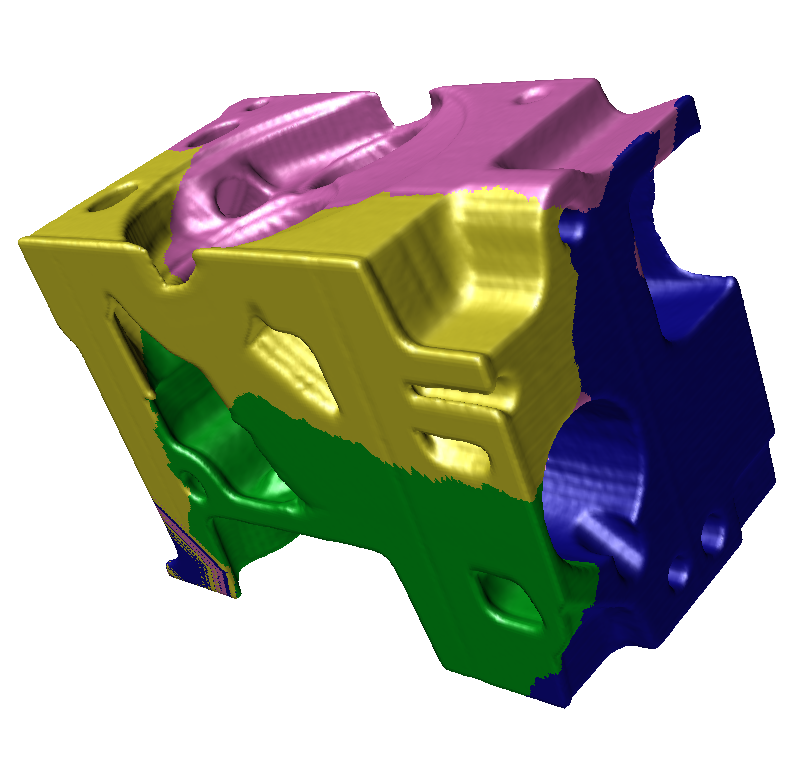
\includegraphics[width=(\textwidth-1cm)/3]
    {images/mt-engine-21.png}}
  \subfloat[back]{
    \label{fig:engine-2}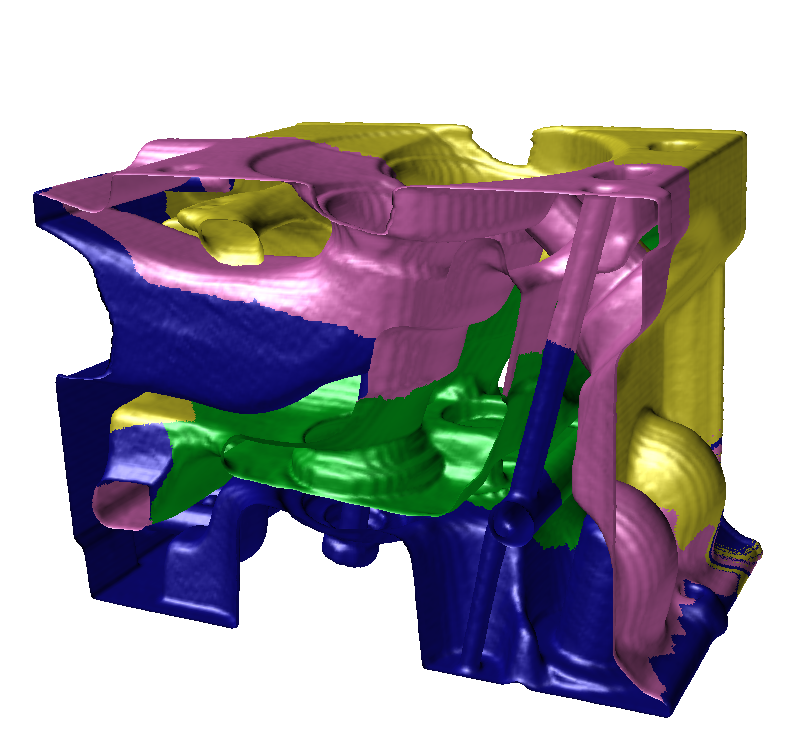
\includegraphics[width=(\textwidth-1cm)/3]
    {images/mt-engine-22.png}}
  \subfloat[side]{
    \label{fig:engine-3}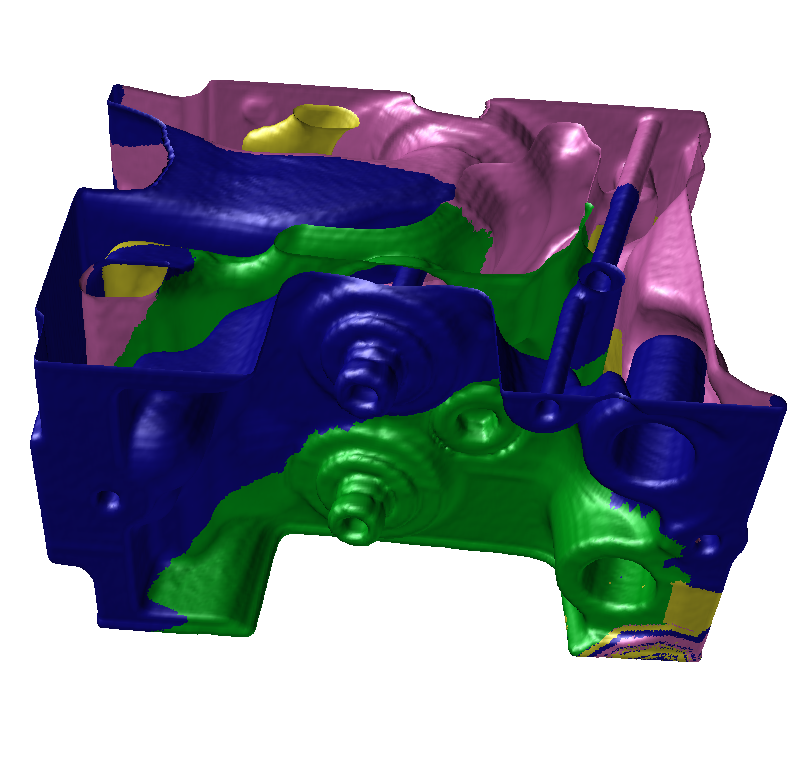
\includegraphics[width=(\textwidth-1cm)/3]
    {images/mt-engine-23.png}}
  \caption[Engine image data with color-tags for threads]
  {A contour component extracted from engine image data,
    where color shows contribution of different processors.}
  % TODO: figure out the NNNs
  \label{fig:engine}
\end{figure}

Results shown in Figure~\ref{fig:engine} indicate that the proposed
algorithm is efficient in assigning work to different threads.
Most of the active cells are continuous because they are extracted using
the same seed cell. The active cells extracted by all threads are almost
equal except for some rare cases when conflict among threads take place.
The conflict might take place on the beginning of the propagation 
due to the starvation among the number of threads. % As is shown on 
% Figure~\ref{fig:mt-sphere-propagate} and Figure~\ref{fig:engine-24},
% starting from the seed on the center, there is a short period time
% that threads competency is very high. On the other hand, however,
% for small contours that extracted using the algorithm, the propagation
% time might be finished within a single thread. 

\begin{figure}[h!]
  \centering
  \subfloat[color-tagged]{
    \label{fig:engine-24}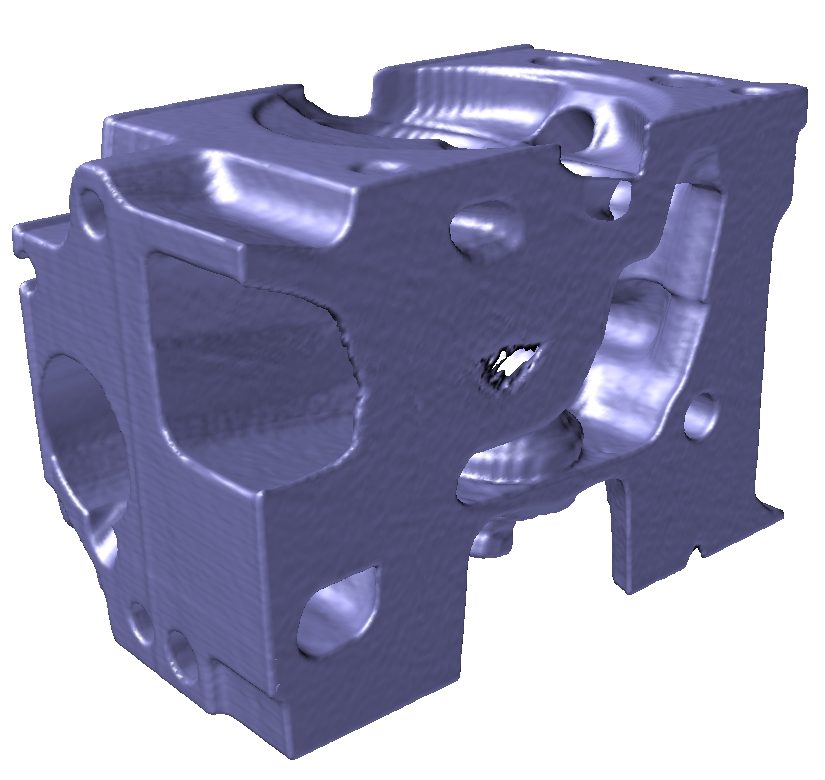
\includegraphics[width=(\textwidth-1in)/2]
    {images/mt-engine2.png}}
  \subfloat[shaded]{
    \label{fig:engine-25}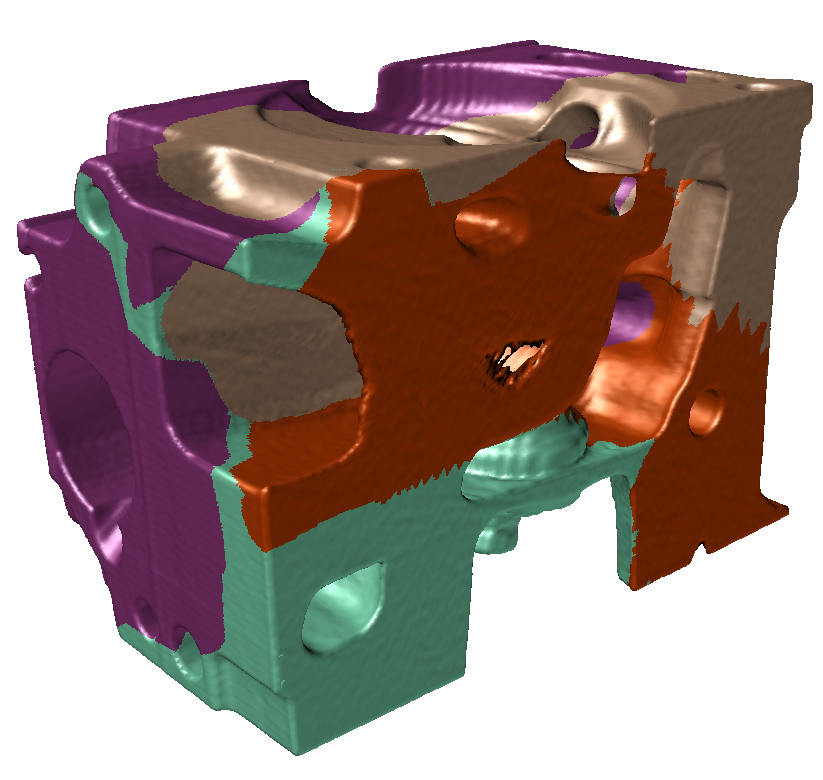
\includegraphics[width=(\textwidth-1in)/2]
    {images/mt-engine1.png}}
  \caption[Comparison between shaded and color-tagged model]
  {Comparison between (\ref{fig:engine-24}) shaded contour component and 
    (\ref{fig:engine-25}) color-tagged model, where slight thread conflict
    take place during initial propagation.}
  \label{fig:shade-engine}
\end{figure}

% \clearpage{}

\begin{figure}[h!]
  \centering
  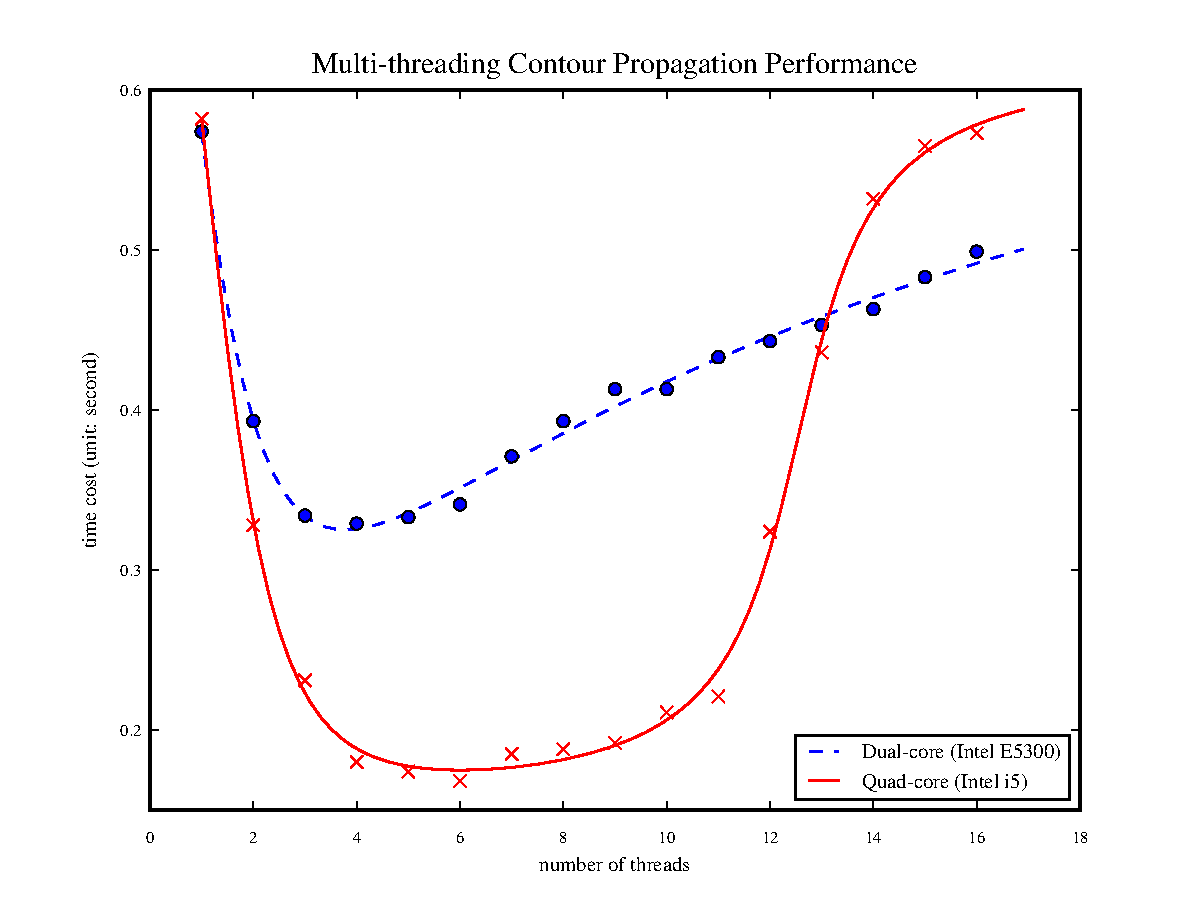
\includegraphics[width=\textwidth-1in]{images/fig-perf-plot.pdf}
  \caption[Multi-threading Contour Propagation Performance]
  {Multi-threading contour propagation performance tested on hemoglobin data.
    ($y$ axis shows time to obtain 1,237,574 tetrahedral cells, while
    lines show fitting function: 
  $f(x) = \frac{\alpha}{x^\beta + \beta x + \gamma} + \delta  arctan (\epsilon  x+\zeta)+\eta$}
  \label{fig:threading1}
\end{figure}

% \begin{figure}[h!] 
%   \centering
%   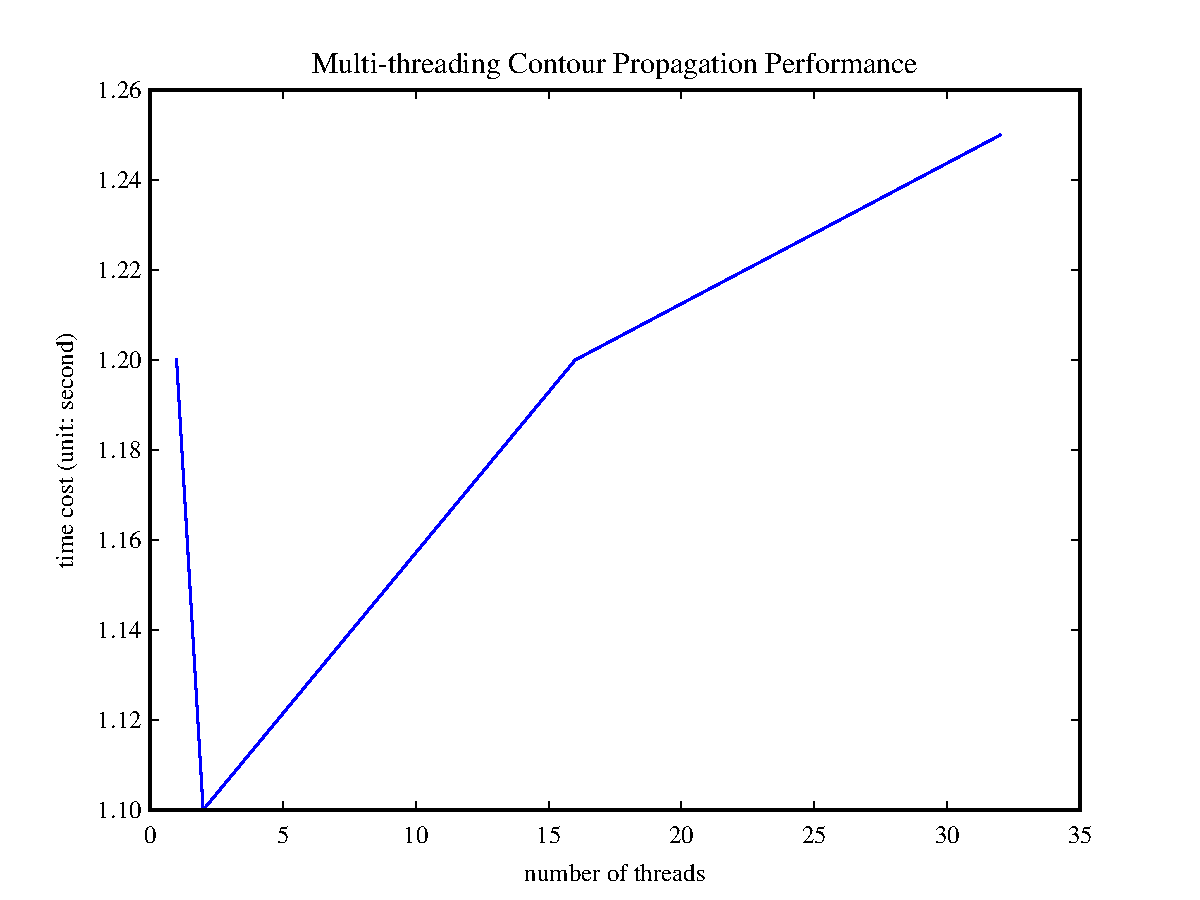
\includegraphics[height=\textheight/4]{images/fig-perf-plot2.pdf}
%   \caption[Multi-threading Contour Propagation Performance]
%   {Multi-threading contour propagation performance tested on hemoglobin data 
%     % (executed on Windows environment with a dual-core processor)
%   }
%   \label{fig:threading2}
% \end{figure}

% \begin{figure}[h!]
%   \centering
%   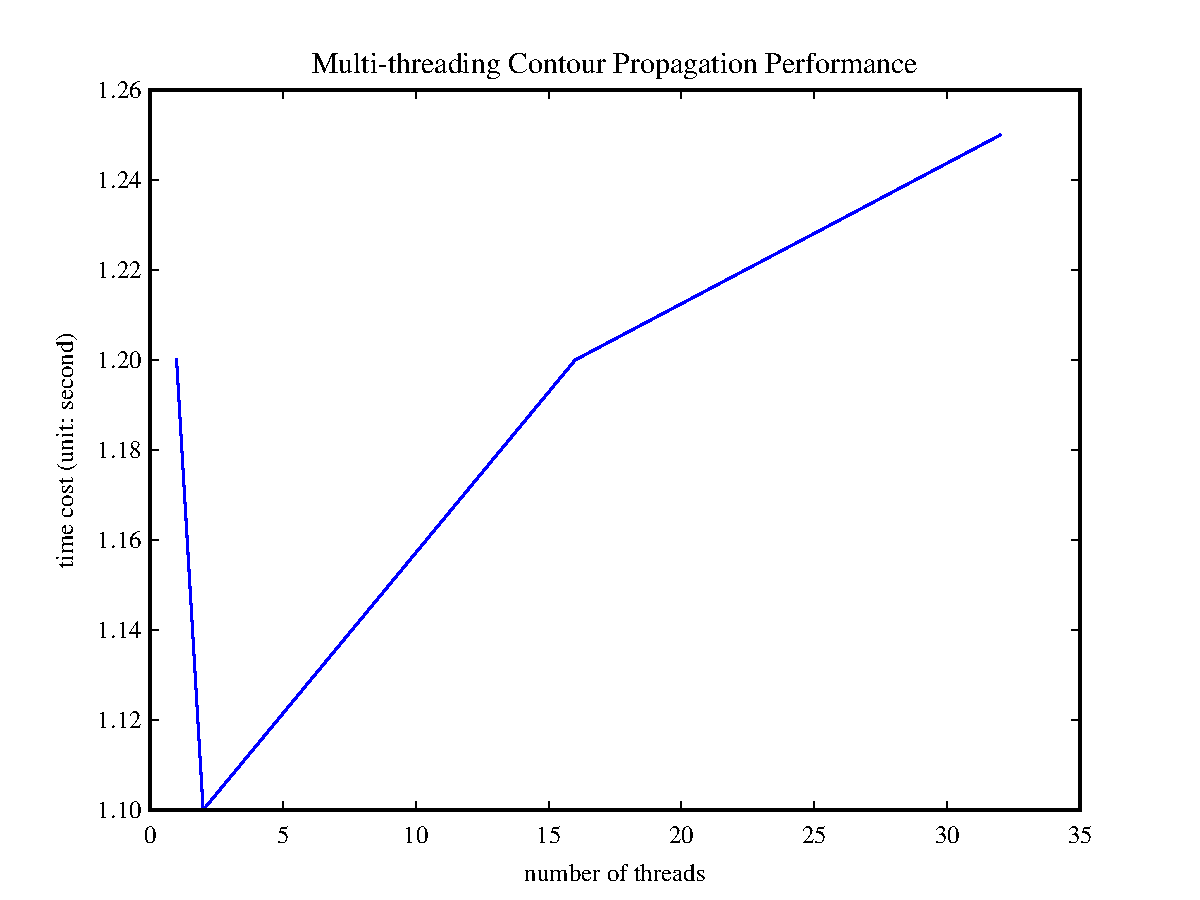
\includegraphics[height=\textheight/4]{images/fig-perf-plot2.pdf}
%   \caption[Multi-threading Contour Propagation Performance 2]
%   {Multi-threading contour propagation performance tested on hemoglobin data 
%     % (executed on Windows environment with a quad-core processor)
%   }
%   \label{fig:threading3}
% \end{figure}

From Figure~\ref{fig:threading1} we can see that when using a dual-core 
processor, best performance can be obtained when using 3$\sim$5 threads.
For the propagation of a large contour, the speedup is much
more efficient using threads more than the number of processors.
This mainly because when conflict take place between two threads, the 
existence of other threads can continue to propagate.
Therefore, the number of threads used in 1.5 times of that of cores to estimate
best performance based on the available hardware.
% Figure~\ref{fig:threading1}% , Figure~\ref{fig:threading2} and 
% Figure~\ref{fig:threading3} 
The figure also shows that starting from using a single 
thread, with the increase of thread use, the time for propagating 
dropped gradually due to the multi-tasking function on different computing units.
% and then gradually drop of the performance due to
% the overhead use of threads that causes conflict between threads.
The drop after obtaining best performance is contributed by overhead host function
calling and too much threads compete to get seeds from shared queue.
But for contours small in size, it's efficient to use threads same as the number 
of processors.

% \begin{figure}[h]
%   \centering
%   \subfloat[Whole Hemoglobin]{
%     \label{fig:hbmatch-1}\includegraphics[width=2.5in]{images/mt-hbmatch-1.png}}
%   \subfloat[Portion]{
%     \label{fig:hbmatch-3}\includegraphics[width=2.0in]{images/mt-hbmatch-3.png}}
%   \caption{Hemoglobin}
%   \label{fig:hbmatch}
% \end{figure}

% \begin{figure}[h]
%   \centering
%   \includegraphics[width=3in]{images/mt-sphere-1}
%   \caption{Sphere}
%   \label{fig:sphere-1}
% \end{figure}
% \clearpage{}

\section{Triangulation Performance}

% Table~\ref{tab:gpuperformance}
GPU performance could be slightly affected by several factors, such as the 
distribution of the GPU processing load, the bandwidth between GPU and CPU, 
as well as memory size in graphics cards.

\paragraph{load balancing}
The distribution of the GPU processing load is assigned by setting the number of 
threads used in each block, which is a multiple of 2. In our experiment, it's
proper to set the value in range from 32 to 128. That is to say that each block 
processes 32$\sim$128 tetrahedral cells at a time, while each cell results in 
1$\sim$2 triangles.
Taking advantage of the \emph{vertex buffer object}(VBO), all these triangles in
the device addresses can be mapped into rendering pipeline by binding buffer 
IDs and enable the vertex buffer in display function.

The amount of work that assigned to each thread are slightly different 
because the number of triangles inside a tetrahedron can be 1 or 2 depending on
the intersection case. The time cost on execution depends on the slowest thread.
Therefore, the time cost in most case is the time consumed on extracting two 
triangles intersected in a single cell.

% It's a significant 
% The bandwidth  
\paragraph{bandwidth}
From Table~\ref{tab:cpuperformance}, we can see that bandwidth is an important 
factor affecting the GPU computing performance. Active cells collected using
multi-tasking should be copied into GPU memory, which is allocated and released
every time. Therefore, data that need to be loaded should be small in size and 
in less frequency. In our experiment, computing cell index on intersection is 
much more efficient than loading precomputed array. Because the computation
on GPU is executed on parallel pipeline, while loading arrays to global 
memory is run in linear time complexity $O(n)$.

\paragraph{miscellaneous}
In practice, CUDA SDK version is another factor that affects the final triangulation
performance. Newer versioned toolkit might be much more optimized to achieve
better performance.

% \begin{itemize}
% \item bandwidth between graphics card : this will affect the data copy
% \item GPU version : newer version of CUDA toolkit might be much more optimized ...
% \item memory size in graphics card : this will affect the mesh size
% \end{itemize}

% The time cost on triangulation can be divided into three parts: combine cells from 
% different threads, GPU memory allocation and copy cell array into graphics card and 
% CUDA kernel execution.

% there are four major step in the GPU program that consume much time:
% \begin{itemize}
% \item memory allocation
% \item time cost when copy active cell array into graphics card
% \item CUDA kernel execution
% % \item rendering time (FPS?)
% \end{itemize}

% Table~\ref{tab:cpuperformance} and Figure~\ref{fig:result-img} shows some tested 
% data, while a comparison chart is given on Figure~\ref{fig:_perf_bar}. These
% results are given to shown that our method improved the 

% \begin{table*}[h]
%   \centering
%   \begin{tabular}{|c|c|c|c|c|c|}
%     \hline
%     data set   & triangles & original method & single thread & two threads & four threads \\
%     \hline
%     % sphere & tri & c & single  & two & four \\
%     fuel & tri & c & single  & two  & four \\
%     skull & tri & c & single  & two & four \\
%     engine & tri & c & single & two & four \\
%     hemoglobin & tri & c & single & two  & four \\
%     ventricle & tri & c & single  & two  & four \\

%     \hline
%   \end{tabular}
%   \caption{GPU Performance}
%   \label{tab:gpuperformance}
% \end{table*}

% \section{Final ROI Visualization}

% Finnally, alpha blending is enabled in order to visualize the hierarchical 
% structure in the volume. ... enable with hybrid accerlated 3D contour 
% extraction.
% ...

\begin{landscape}
  \begin{table*}[h]
    \centering
    \begin{tabular}{|c|c|c|c|c|c|c|c|c|c|c|}
      \hline
      \multirow{2}{*}{data set} & \multirow{2}{*}{dimension} & \multirow{2}{*}{triangles} & \multirow{2}{*}{active cells} & \multirow{2}{*}{previous} & \multicolumn{2}{|c|}{propagation}  & \multicolumn{2}{|c|}{triangulation} & \multirow{2}{*}{proposed} & \multirow{2}{*}{speedup} \\ \cline{6-9}
              &  &  &  &  & \multirow{1}{*}{original} & \multirow{1}{*}{proposed} & \multirow{1}{*}{original} & \multirow{1}{*}{proposed} & & \\
      \hline
      % sphere & dim & tri & cell &  seq & 2thr & 4thr & cuda \\
      % hand & dim & tri & cell &  seq & 2thr & 4thr & cuda \\
      fuel        & 64x64x64 & 33618 & 25613 & 0.0984 & 0.016 & 0.009 & 0.056 & 0.007 & 0.0165 & x5.96  \\
      % skull & dim & tri & c & o & four & cu \\
      visible human & 128x128x128 & 471107 & 357986 & 1.0545 & 0.220 & 0.053 & 0.829 & 0.086 & 0.1517 & x6.95 \\
      head        & 128x128x128 & 573840 & 436870 & 1.2250 & 0.264 & 0.058 & 0.955  & 0.103 & 0.1745 & x7.02 \\
      kidney      & 128x128x128 & 769305 & 586956 & 1.7316 & 0.362 & 0.086  & 1.364  & 0.138 & 0.2417 & x7.16 \\
      hemoglobin  & 128x128x128 & 1619392 & 1235133 & 3.626 & 0.763 & 0.194 & 2.856 & 0.294 & 0.524 & x6.9 \\
      ventricle   & 256x256x128 & 643171 & 491264 & 1.5214 & 0.312 & 0.069 & 1.172  & 0.118 & 0.2334 & x6.52 \\
      engine      & 256x256x128 & 2060552 & 1561463 & 4.6664 & 0.986 & 0.212 & 3.639  & 0.369 & 0.6580 & x7.09 \\
      % foot & dim & tri & cell &  seq & 2thr & 4thr & cuda \\
      % MRIHead & dim & tri & c & o & four & cu \\
      \hline
    \end{tabular} 
    \caption[Performance Analyzing Table]{Performance Analyzing Table 
      (In order to prove the efficiency of the proposed algorithm, we selected large contours in the dataset for
  testing the performance.)
      % (data in CUDA shows the allocation time, execution time and memory releasing time respectively.)
    }
    % \begin{tabular}{|c|c|c|c|c|c|c|c|}
    %   \hline
    %   data set & dimension & triangles & active cells & sequential & 2 threads & 4 threads & CUDA \\
    %   \hline
    %   sphere & dim & tri & cell &  seq & 2thr & 4thr & cuda \\
    %   fuel        & 64x64x64 & 33618 & 25613 & 0.019s & 0.011s & 0.012s & 0.0011+0.000030+0.0008 \\
    %   % skull & dim & tri & c & o & four & cu \\
    %   vh4 & 128x128x128 & 471107 & 357986 & 0.271s & 0.149s & 0.150s & -- \\
    %   head      & 128x128x128 & 573840 & 436870 & 0.331s & 0.219s & 0.186s & -- \\
    %   kidney & 128x128x128 & 769305 & 586956 & 0.452s & 0.287s & 0.257s  & 0.0135+0.000031+0.0082 \\
    %   hemoglobin  & 128x128x128 & 1619392 & 1235133 & 0.929s & -- & 0.513s & 0.0267+0.000048+0.0169
    %   \\
    %   ventricle   & 256x256x128 & 643171 & 491264 & 0.372s & -- & 0.212s & 0.0114+0.000051+0.0066 \\
    %   engine      & 256x256x128 & 2060552 & 1561463 & 1.201s & -- & 0.676s & -- \\
    %   % foot & dim & tri & cell &  seq & 2thr & 4thr & cuda \\
    %   % MRIHead & dim & tri & c & o & four & cu \\
    %   \hline
    % \end{tabular} 
    % \caption[Performance Analyzing Table]{Performance Analyzing Table 
    %   (data in CUDA shows the allocation time, execution time and memory releasing time respectively.)}
    \label{tab:cpuperformance}
  \end{table*}

  
    
\end{landscape}

% \begin{landscape} 
\begin{figure}[H]
  \centering
  \subfloat[fuel]{
    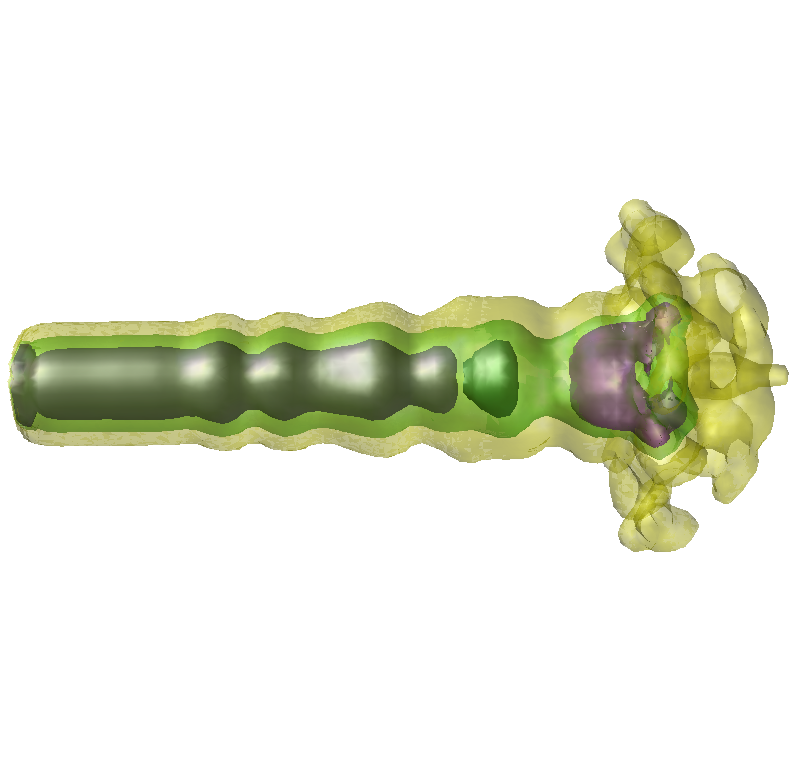
\includegraphics[height=(\textheight-2in)/3]{images/result2-fuel}
    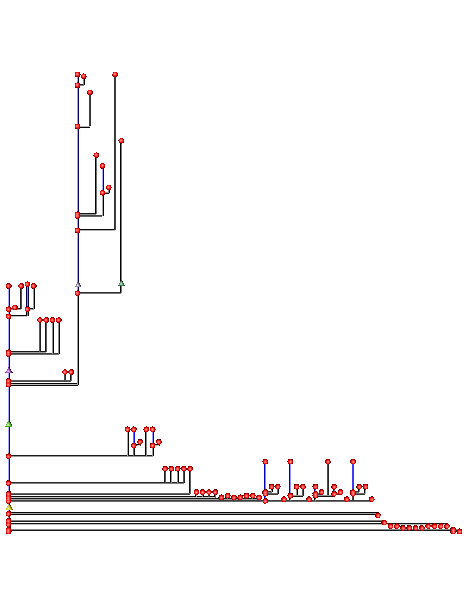
\includegraphics[height=(\textheight-2in)/3]{images/result2-fuel-tree}}\\
  \subfloat[head]{
    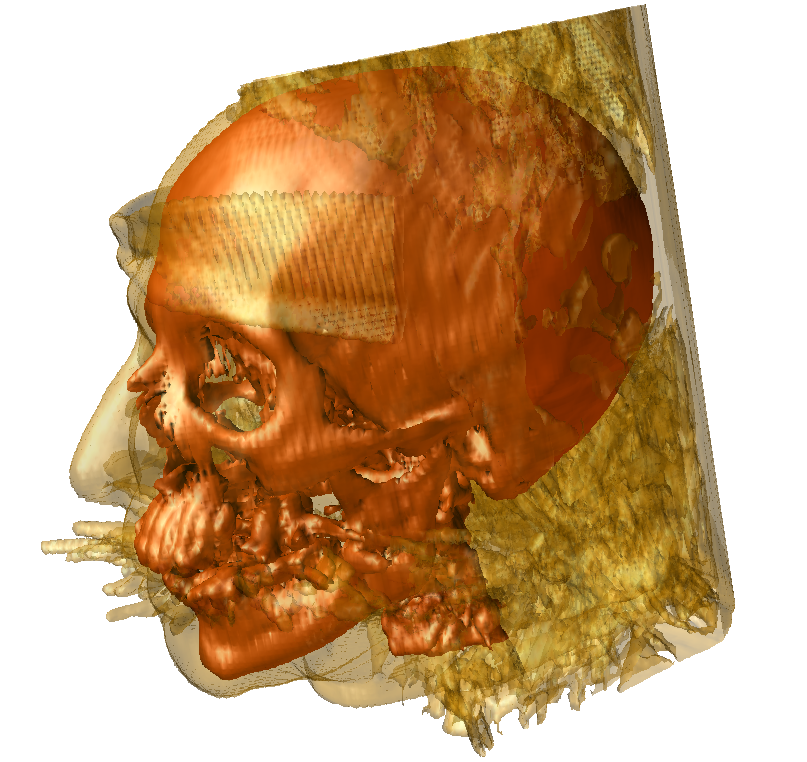
\includegraphics[height=(\textheight-1in)/3]{images/result2-head}
    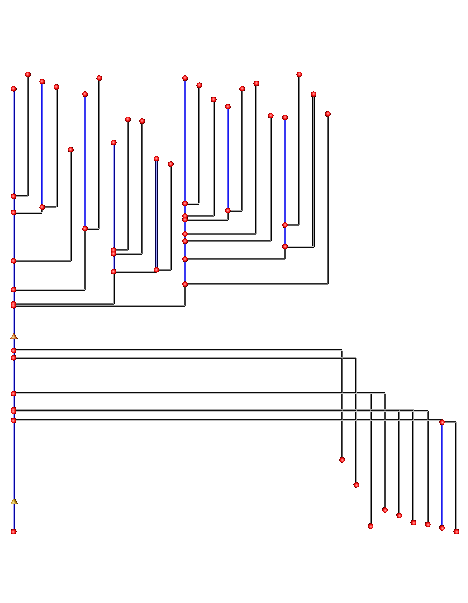
\includegraphics[height=(\textheight-1in)/3]{images/result2-head-tree}}\\
  \subfloat[engine]{
    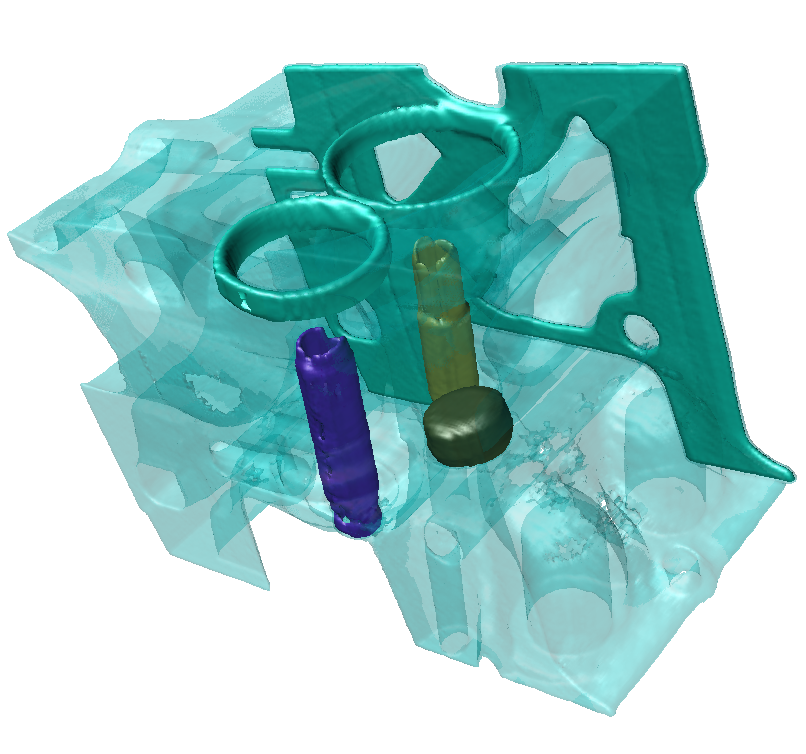
\includegraphics[height=(\textheight-1in)/3]{images/result2-engine}
    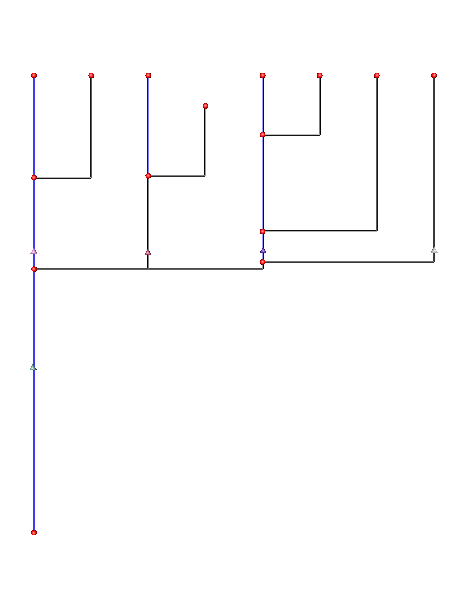
\includegraphics[height=(\textheight-1in)/3]{images/result2-engine-tree}}
  \caption{Final results}
  \label{fig:result-img1}
\end{figure}

\begin{figure}[H]
  \centering
  \subfloat[visible human]{
    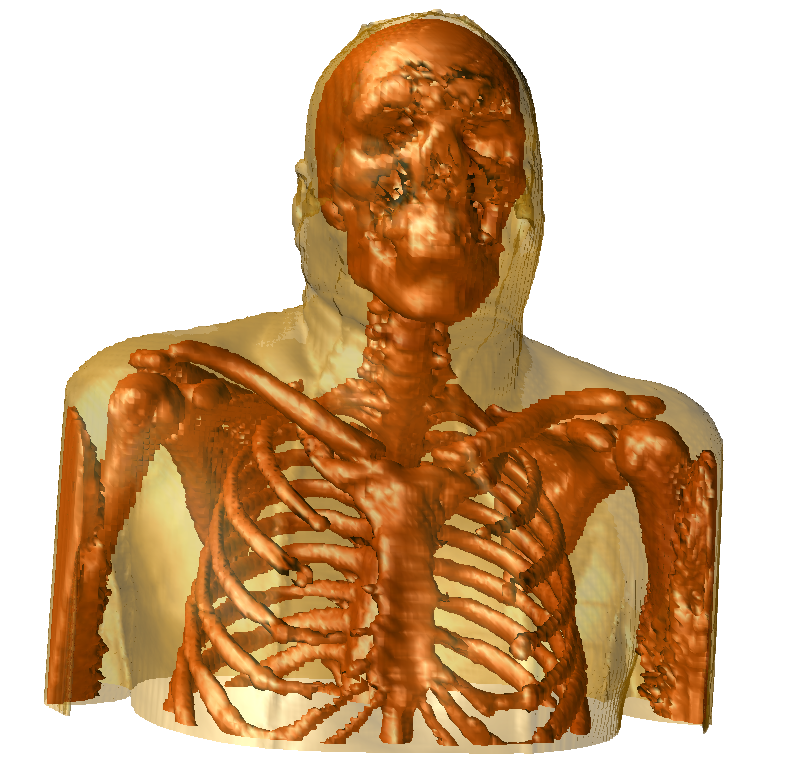
\includegraphics[height=(\textheight-1in)/3]{images/result2-vh4}
    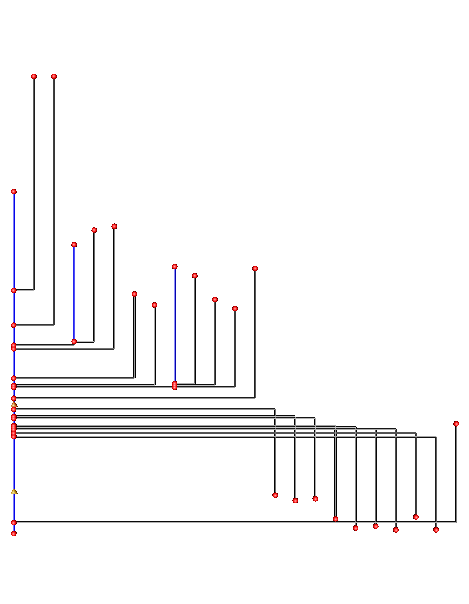
\includegraphics[height=(\textheight-1in)/3]{images/result2-vh4-tree}}\\
  \subfloat[kidney]{
    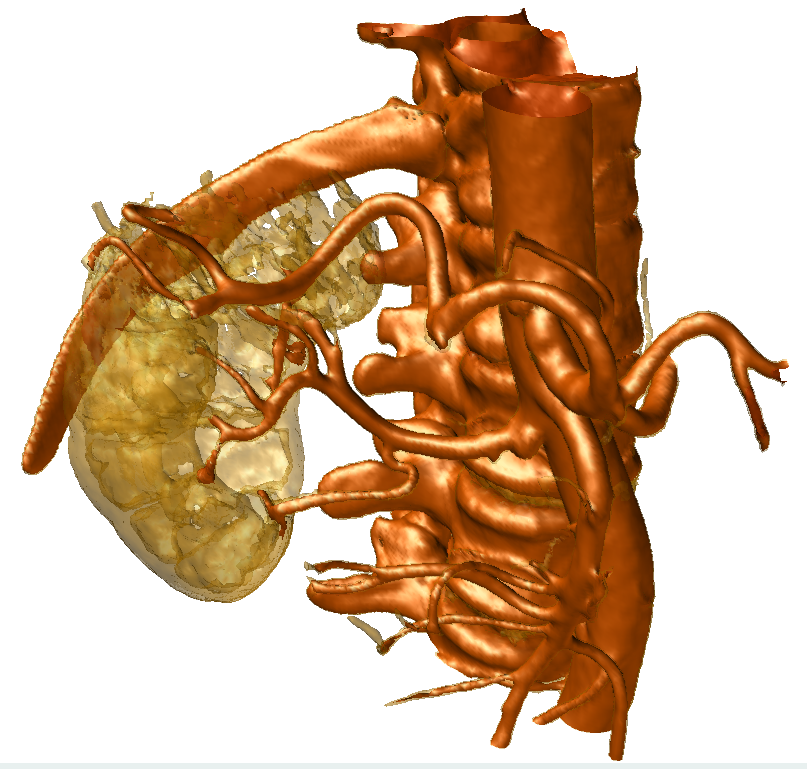
\includegraphics[height=(\textheight-1in)/3]{images/result2-kidney}
    \includegraphics[height=(\textheight-1in)/3]{images/result2-kidney-tree}}\\
  \subfloat[hemoglobin]{
    \includegraphics[height=(\textheight-1in)/3]{images/result2-hemoglobin}
    \includegraphics[height=(\textheight-1in)/3]{images/result2-hemoglobin-tree}}
  \caption{Final results}
  \label{fig:result-img2}
\end{figure}

% We have experimented using various data vary from tiny synthesized molecule data to
% large human body parts.

% \end{landscape}


%-----------------------------------------------------------------------------
% \include{conc}
\chapter*{Chapter 6. Conclusions and Future Works}
\addcontentsline{toc}{chapter}{Chapter 6. Conclusions and Future Works}
\setcounter{tocdepth}{0}
\setcounter{chapter}{6}
\setcounter{section}{0}
\label{ch:conc}

This thesis aim to take the advantage of modern hardware to extract the 
interesting information in 3D volume data. To address the problem of finding
contours of interest, we construct contour tree and use it as the visual 
representation of the data. To apply the method to large data with noisy 
structures, hierarchical simplification algorithm is applied the the 
contour tree. Hence, an interface is created to enable the interaction 
to map the structure to surface mesh. The hybrid algorithm proposed 
in this thesis improved the mapping action significantly 
by threaded propagation in CPU and GPU accelerated triangulation.

The reason to use CPU for the propagating operation mainly because it is 
implemented with heavy conditional controls. Multi-core CPUs got its
advantage to manage these operation with highly developed thread 
synchronization functions, which is not yet enabled in GPU programming.

% From the performance chart Figure~\ref{fig:threading}, 

In this thesis, an assumption was made that the input data should 
be simplicial mesh. The application is limited to result in rectangular
geometry mesh.

We want to continue this work by using more statistical information in the 
volume data to show salient contours in an interactive way. Besides, 
view-dependent method can be applied to improve the extraction speed 
by propagating only the surface face to the view-point. Other future
improvements include the possible to implement efficient propagation
method on GPU and developing proper volume dividing method to enable
the application to large dataset.

% list of future improvement:
% \begin{itemize}
% \singlespacing
% \item cubic triangulation in CUDA
% \item enable volume large data loaded on CUDA memory instead of data 
% preloading
% \end{itemize}

% \section{Discusion}

% \section{Summary}

% \section{Future Works}
% \subsection{Saliency Computation}
% \setcounter{page}{35}
\cleardoublepage
\addcontentsline{toc}{chapter}{Reference}
\renewcommand{\bibname}{Reference}
\bibliographystyle{plain}
% \bibliographystyle{alpha}
\bibliography{thesis}

% \chapter{Korean Abstract}

\setcounter{page}{37}
\clearpage
\setcounter{page}{38}
\addcontentsline{toc}{chapter}{국문초록}
\includepdf{abstract-kr.pdf}
% \chapter{English Abstract}
\setcounter{page}{39}
\addcontentsline{toc}{chapter}{Abstract}
\includepdf{abstract-en.pdf}

\end{document}
